\section{Python Interpreters}\label{sec:pythoninterpreters}
%%% note : add this to the section of python interpreters
Due to the lack of support for most non-conventional Python interpreters, we mainly focus on micro-benchmarks.
Except for \textsc{PyPy}, most of the Python implementations do not support extra Python libraries, despite those extra implementations being developed to optimize a specific library, such as \textsf{Numba} with \textsf{Numpy}, or \textsf{intelpython} with machine learning algorithms.


\paragraph{Preliminary studies}
For the first studies, we used the official version of Python, because the goal was mainly to highlight the impact of the structure of code on energy consumption.
One main drawback of the previous method is the work to be done to update the existing code base to reduce  energy consumption.
To avoid such hustle, we tried to find a non-intrusive approach to make the Python code more eco-friendly without altering its structure.
Python is an interpreted language, which led many initiatives to implement their own interpreter to improve one or many aspects of the Python code.
In the following section, we discuss the impact of those implementations on the energy consumption of python programs, and in which case, one should use a non-conventional interpreter to save the energy consumption of their application.

To do so, we gathered a list of interpreters, transpilers and other optimization libraries that can contribute to reduce the energy consumption of legacy Python applications:
\begin{enumerate}
      \item \textbf{CPython}:\footnote{\url{https://www.python.org/}}
            This Python interpreter, written in C, is the reference interpreter of Python.
            CPython compiles the source code into byte-code and then interprets it.
            The CPython project supports both versions of Python 2 and 3;
      \item \textbf{PyPy}:\footnote{\url{http://pypy.org}}
            An alternative implementation of the Python interpreter.
            It is written using \emph{RPython} to use the JIT.
            It compiles the most used portions of the Python code into a binary code for better performance.
            To benefit from these optimizations, the program has to be executed for at least for few seconds so the JIT has enough time to warm up, the JIT optimization are only applied to the code written by the developer and not to external libraries;
      \item \textbf{Cython}:\footnote{\url{https://github.com/cython/cython}}
            A static compiler for Python.
            It translates the Python code into C, and then compiles it using a C compiler.
            It also supports an extended version of the Python language that allows programmers to call \emph{C functions}, declare \emph{C types} and use static types, which will help the translation of Python objects into native types, such as integers, float.
            This often means better performances, since native C libraries are almost all the time faster than the Python written once~\cite{pereira_energy_2017};
      \item \textbf{Intel\,Python}:\footnote{\url{https://software.intel.com/en-us/distribution-for-python}}
            A customized interpreter developed by Intel to enhance performances of Python programs.
            It is dedicated to data sciences and high-performance computing.
            It uses some Intel kernel libraries, such as Math Kernel Library (Intel MKL\footnote{\url{https://software.intel.com/en-us/mkl}}) and data analytics acceleration library (Intel DAAL\footnote{\url{https://software.intel.com/en-us/intel-daal}}).
            It supports both versions of Python;
      \item \textbf{Active\,Python}:\footnote{\url{https://www.activestate.com/products/activepython/}}
            It is developed by the Activestates company and provides a standardized Python distribution to ensure license compliance, security, compatibility and performance.
            Therefore, ActivePython implements its built-in packages (more than 300 packages) and supports both versions of Python;
      \item \textbf{IronPython}:\footnote{\url{https://ironpython.net}}
            A .Net-based Python interpretation platform written in C\# that is used with the .Net virtual machine or Mono.
            It benefits from all the optimizations of .Net virtual machines, such as the JIT and garbage collector mechanisms;
      \item \textbf{GraalPython}:\footnote{\url{https://github.com/graalvm/graalpython/}}
            A Python interpreter that is based on GraalVM\footnote{\url{https://www.graalvm.org/docs/why-graal/}} (a universal virtual machine developed by oracle for running applications written in different programming languages).
            For the time being, it only supports Python~3 and it is still in the experimental stage;
      \item \textbf{Jython}:\footnote{\url{https://jython.github.io}}
            An implementation of Python programming language written in Java for the \emph{Java Virtual Machine} (JVM).
            Similar to IronPython and GraalPython, it leverages the optimization mechanisms provided by the JVM to enhance the Python performances;
      \item \textbf{MicroPython}:\footnote{\url{http://micropython.org}}
            A lightweight Python version dedicated to embedded systems and micro-controllers;
      \item \textbf{Nuitka}:\footnote{\url{http://nuitka.net/pages/overview.html}}
            A Python compiler written in Python that generates a binary executable from Python code.
            It translates the Python code into a C program that is then compiled into a binary executable;
      \item \textbf{Numba}:\footnote{\url{https://numba.pydata.org}}
            A library that includes JIT compiler to enhance the performances of Python functions using the industry-standard LLVM compiler library;
      \item \textbf{Shedskin}:\footnote{\url{https://github.com/shedskin/shedskin}}
            A static transpiler that translates implicitly statically typed python into C++ code;
      \item \textbf{Hope}~\cite{akeret_hope_2015}:
            A Python library that aims to introduce JIT compiler into the Python code;
      \item \textbf{Parakeet}~\cite{DBLP:conf/hotpar/RubinsteynHWS12}:
            A runtime accelerator for an array-oriented subset of Python;
      \item \textbf{Stackless\,Python}:\footnote{\url{https://github.com/stackless-dev/stackless/wiki}}
            An interpreter that focuses on enhancing multi-threading programming;
      \item \textbf{Pyjion}:\footnote{\url{https://github.com/microsoft/pyjion}}
            A JIT API for CPython, same purpose as Parakeet and Hope;
      \item \textbf{Pyston}:\footnote{\url{https://blog.pyston.org}}
            A performance-oriented Python implementation built using LLVM and modern JIT techniques.
            The project is funded by Dropbox;
      \item \textbf{Grumpy}:\footnote{\url{https://github.com/google/grumpy}}
            A source-to-source transpiler that translates the Python code into Go before being compiled to a binary executable.
            It also offers an interpreter, called \emph{grumprun}, which can directly execute the Python code.
            Unfortunately, we cannot use it because the project is already outdated (last commit is in 2017) and it has a lot of limitations in terms of supporting the Python language, such as some built-in functions and standard libraries;
      \item \textbf{Psyco}:\footnote{\url{http://psyco.sourceforge.net}}
            A JIT compiler for Python;
      \item \textbf{Unladen\,Swallow}:\footnote{\url{https://unladen-swallow.readthedocs.io/en/latest/}}
            An attempt to (use) LLVM as a JIT compiler for CPython.
\end{enumerate}


\subsection{Runtime Classification}
Before further proceeding with the list of candidate runtime for Python applications, we propose a classification according to several criteria:
\begin{description}
      \item[\bf Type] refers to the category of runtime infrastructure that supports the execution of a Python application.
            In particular, we consider 3 types of environments: \emph{Interpreter}, \emph{Compiler} and \emph{Library};
            \emph{Interpreter} refers to the class of environment that does not require any preprocessing of Python source code;
            \emph{Compiler} introduces a compilation phase before the execution of the application.
            Finally, \emph{Library} requires some modification of the source code;
      \item[\bf Runtime] refers to the technology supporting the execution of a Python application.
            This technology can refer to the programming language used to program the interpreter, the target language for a compiler or a library;
      \item[\bf JIT optimization] refers to the support of \emph{just-in-time} compilation in the runtime infrastructure supporting the execution of the application;
      \item[\bf GC optimization] refers to the support of \emph{garbage collection} in the runtime infrastructure supporting the execution of the application;
      \item[\bf Python version(s)] refers to the list of Python source code versions supported by the runtime environment.
\end{description}

We should explain the classification of these runtimes
\begin{table}
      \caption{Classification of Python implementations}
      \label{fig:python-classes}
      \small
      \center
      \begin{tabular}{|l|c|c|c|c|c|c|}
            \hline
            \multirow{2}{*}{\bf Name} & \multirow{2}{*}{\bf Type} & \multirow{2}{*}{\bf Runtime} & \multicolumn{2}{c|}{\bf Optimisations} & \multicolumn{2}{c|}{\bf Python}                     \\
            % \cline{1-5}
                                      &                           &                              & {\bf JIT}                              & {\bf GC}                        & {\bf 2} & {\bf 3} \\
            \hline
            \hline
            CPython                   & Interpreter               & C                            & \no                                    & \no                             & \yes    & \yes    \\
            \hline
            Intel\,Python             & Interpreter               & C                            & \no                                    & \no                             & \yes    & \yes    \\
            \hline
            ActivePython              & Interpreter               & C                            & \no                                    & \yes                            & \yes    & \yes    \\
            \hline
            PyPy                      & Interpreter               & Python                       & \yes                                   & \yes                            & \yes    & \yes    \\
            \hline
            IronPython                & Interpreter               & .Net                         & \yes                                   & \yes                            & \yes    & \yes    \\
            \hline
            GraalPython               & Interpreter               & GraalVM                      & \yes                                   & \yes                            & \no     & \yes    \\
            \hline
            Jython                    & Interpreter               & Java                         & \yes                                   & \yes                            & \yes    & \no     \\
            \hline
            Stackless\,Python         & Interpreter               & Python                       & \no                                    & \no                             & \yes    & \no     \\
            \hline
            MicroPython               & Interpreter               & c                            & \no                                    & \no                             & \no     & \yes    \\
            \hline
            Pyston                    & Interpreter               & LLVM                         & \yes                                   & \no                             & \yes    & \no     \\
            \hline
            Unladen\,Swallow          & Interpreter               & LLVM                         & \yes                                   & \no                             & \yes    & \no     \\
            \hline
            \hline
            Cython                    & Compiler                  & C                            & \no                                    & \no                             & \yes    & \yes    \\
            \hline
            Nuitka                    & Compiler                  & C                            & \no                                    & \no                             & \yes    & \yes    \\
            \hline
            Shedskin                  & Compiler                  & C++                          & \no                                    & \no                             & \yes    & \yes    \\
            \hline
            Grumpy                    & Compiler                  & Go                           & \no                                    & \no                             & \yes    & \yes    \\
            \hline
            \hline
            Numba                     & Library                   & C                            & \yes                                   & \no                             & \yes    & \yes    \\
            \hline
            Hope                      & Library                   & Python                       & \yes                                   & \no                             & \yes    & \yes    \\
            \hline
            Psyco                     & Library                   & Python                       & \yes                                   & \no                             & \yes    & \yes    \\
            \hline
            Pyjion                    & Library                   & .NET Core                    & \yes                                   & \no                             & \yes    & \yes    \\
            \hline
            Parakeet                  & Library                   & C                            & -                                      & \no                             & \yes    & \no     \\
            \hline
      \end{tabular}
\end{table}



\begin{table}[hbt]
      \caption{Classification of Python implementations}
      \label{fig:pythonimplementations}
      \small
      \center
      \begin{tabular}{|l|c|c|c|}
            \hline
            Version  & Interpreter     & Transpiler/Compiler & Jit library \\
            \hline
            \hline
            Python~2 & Cpython2        & Cython2             & Numba 2     \\
            % \cline{2-4}
                     & Pypy2           & Shesdskin           & Hope        \\
            % \cline{2-4}
                     & Pyston          & Grumpy              & Parakeet    \\
                     & Ironpython      &                     & Psyco       \\
                     & Jython          &                     & Pyjion      \\
            % &  &  &  \\
                     & Micropython     &                     &             \\
                     & Pysec           &                     &             \\
                     & StacklessPython &                     &             \\
            % \cline{2-4}
            \hline
            Python~3 & Cpython3        & Nuitka              & Numba3      \\
                     & Pypy3           &                     &             \\
                     & GraalPython     &                     &             \\
            \hline
      \end{tabular}
\end{table}

There are other implementations that we did not consider because either the project aborted many years ago or it has very limited support for Python features.
After the inventory of those implementations, we filtered them.
To keep only the versions that are still maintained and support most Python features.
We then classified them into 3 categories depending on their integration with the Python code.
In \Cref{fig:pythonimplementations}, we describe the implementations that we kept, the version of each implementation and its category.

\begin{figure}
      \centering
      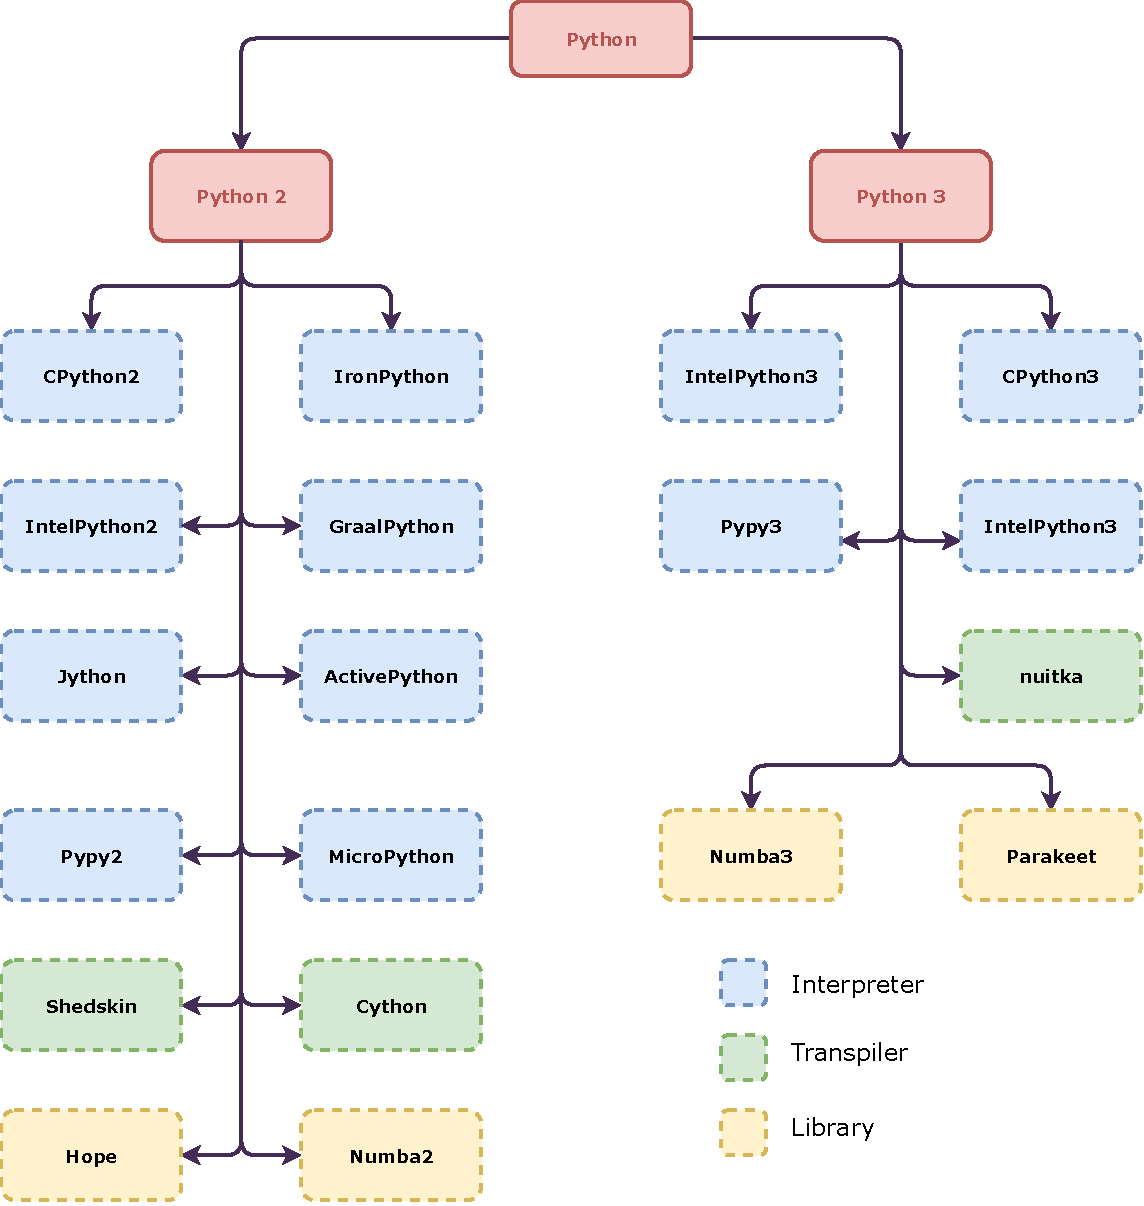
\includegraphics[width=.7\linewidth]{imgs/python-implementations-tree}
      \caption{Python interpeters}
      \label{fig:interpreters}
\end{figure}



\section{Experimental Protocol}
As discussed in the previous chapter, our idea is to design a benchmarking solution that allows practitioners to reproduce and extends our benchmarks.
This benchmarking solution is also the one we use to answer the research questions addressed in this manuscript.
%%%% probably ill resue the same things from other chapters

\subsection{Measurement Context}
\paragraph{Hardware settings.}
All our benchmarks have been executed on a Dell PowerEdge C6420 server, whose hardware features are summarized in Table~\ref{fig:dahuconfig}.
The server uses a minimal version of Debian\,9 (4.9.0 kernel version) where we install Docker (version 18.09.5).

\begin{table}[hbt]
      \resizebox*{\linewidth}{!}{
            \begin{tabular}{ll}
                  \hline
                  CPU     & Intel Xeon Gold 6130 (Skylake, 2.10GHz, 2 CPUs/node, 16 cores/CPU)                                                     \\
                  Memory  & 192 GiB                                                                                                                \\
                  Storage & 240 GB SSD SATA Samsung MZ7KM240HMHQ0D3                                                                                \\
                          & 480 GB SSD SATA Samsung MZ7KM480HMHQ0D3                                                                                \\
                          & 4.0 TB HDD SATA Seagate                                                                                                \\
                  Network & eth0/enp24s0f0, Ethernet, configured rate: 10 Gbps, model: Intel Ethernet Controller X710 for 10GbE SFP+, driver: i40e \\
                          & ib0, Omni-Path, configured rate: 100 Gbps, model: Intel Omni-Path HFI Silicon 100 Series [discrete], driver: hfi1      \\
                  \hline
            \end{tabular}
      }
      \caption{Benchmarking server configuration.}
      \label{fig:dahuconfig}
\end{table}

\paragraph{Software settings.}
For the sake of reproducibility, each experiment runs within a Docker container.
\subsection{Key Performance Metrics}
Our focus will be mainly on CPU energy consumption as it is ten folds more than the DRAM one, since it is a task-based benchmarking, time is highly correlated within the energy, and it will be only useful to explain some specific energy behaviors, thus we do not put a lot of focus on this metric.
%% basically i what i want to say is that we we care mostly about energy, because there are studies that were made on the performance, plus the DRAM is not that interested even within the heavy memory  benchmakrs

\paragraph{Energy measurement.}
As we know, the energy of a program is integral of its power over time.
For our case, we used Intel \emph{Running Power Average Limit} (RAPL)~\cite{Khan:2018:RAE:3199681.3177754} to collect the power samples of the running tests.
We run \textsc{PowerAPI}~\cite{DBLP:journals/jss/ColmantRKSFS18}, to report on measurements collected by Intel RAPL and upload them to a so-called \emph{computing machine}, then we calculate the Energy using the trapezoidal rule:
% \begin{figure}[hbt]
% \centering
\begin{equation}
      E = \int^a_b P(t)dt \simeq \sum^n_{k=1} \frac{P(t_k-1)+P(t_k)}{2}
\end{equation}
% \caption{}
% \label{fig:trapezrule}
% \end{figure}
Figure~\ref{fig:powerapi} overviews the architecture of our benchmarking infrastructure.

\begin{figure}[hbt]
      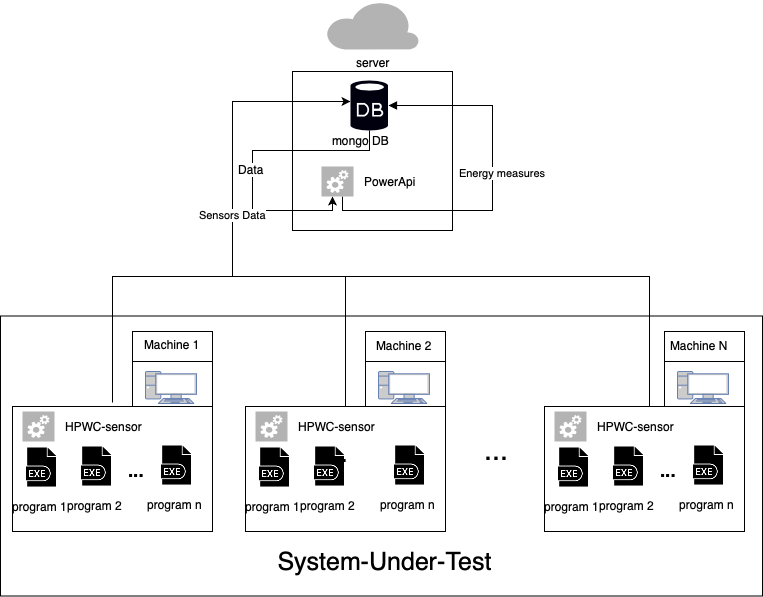
\includegraphics[width=.9\linewidth]{imgs/SmartWatts.png}
      \caption{Benchmarking architecture deployed with \textsc{PowerAPI}.}
      \label{fig:powerapi}
\end{figure}

The motivation for separating measurement collection from energy computations is to reduce any interference with the benchmark, our sensor being a lightweight C program running as a Docker container.

\subsection{Benchmark Preparation}
\paragraph{Input workload.}
To benchmark our implementations, we employed the \textsc{Tommti} microbenchmarks suite.\footnote{\url{http://www.tommti-systems.de/main-Dateien/reviews/languages/benchmarks.html}}
\textsc{Tommti} is a set of 13 microbenchmarks that examine common language features, such as arithmetic operations, data structures and input/output manipulations, among others.
In addition to these microbenchmarks, we implemented some binary operations to investigate the behavior of the previous implementations when it comes to low-level operations that only works with registries.

To study the energy behavior of the Python implementations, we have to focus on the effect of the implementations and mitigate any side effect, such as the organization of the code or any extra consumption due to the operating system or third-party libraries.
Therefore, for each benchmark, we took the implementation written in Python2 as a reference and tried to use it in other implementations as it is.
If it is not supported by Python3, we converted the code using the official library \emph{2to3}.\footnote{\url{https://docs.python.org/3.7/library/2to3.html}}
In the case of the libraries using \emph{JIT} adding a decorator to the function that we want to optimize was enough, if there are other changes, we assume that they alter the original code which is against our purpose.
Each benchmark is isolated in a Docker container for several reasons:
\begin{itemize}
      \item Isolation: each container has only the benchmark program implemented with a single python runtime to remove any interference between different implementations,
      \item Deployment: to use the benchmarking machine without extra configurations that may alter the behavior of the operating system toward energy consumption,
      \item Reproducibility: one of the most frequent benchmark crimes~\cite{DBLP:journals/corr/abs-1801-02381} in research is the lack of reproducibility---by using Docker we ensure that each benchmark has an image that will be publicly accessible.
\end{itemize}

Despite the presence of the official docker images for most of the runtimes, we preferred to build our own using the same reference image to remove any bias due to the OS used in the official images.
We used ArchLinux with kernel version 4.9.184 as a base image for all our benchmarks.

\paragraph{Benchmark extension.}
As we have done with the previous chapters, we provide a tool that allows extending the benchmarks with new workloads and new candidates.
In the repository listing the Python implementations under study,\footnote{\url{https://github.com/chakib-belgaid/python-implementations}} we propose a dedicated tool to generate new workloads and new candidates.
The script \texttt{generator.py} allows practitioners to create new benchmarks by implementing a Python code within different interpreters.
Then, it generates \texttt{launcher-benchmark.sh} that can be executed to run the associated benchmark.
Furthermore, all the successful implementations are stored in a separate directory and the ones that failed (\emph{e.g.}, mostly because of compatibility issues) are stored in a recap file called \texttt{benchmarkTest.md}, where \texttt{benchmark} is the name of the new workload.
To add new candidate runtimes, one should add a base Docker file that contains the new implementation and, if there should be extra manipulation that should be added to the workload files such as adding new decorator or changing some parameters, then they should be added as an extra function in the script \texttt{generator.py}.
Finally, they should be included in the Python candidates.

\section{Results \& Findings}
This section will be dedicated to the results of the experiments and statistical analysis of these results.
Because we are conducting a comparison study, we first did a Shapiro-Wilk~\cite{shapiro1968comparative} test to see if the data follows a normal distribution.
Despite the fact that some implementations had a $p$-value higher than $a=0.05$ (such as CPython and ActivePython), other implementations like PyPy and Numba presented a $p$-values smaller than 0.01, which leads to reject the hypothesis $H0$ that all the distributions follow a normal distribution.
Therefore, to compare the different implementations, we performed the non-parametric Mann-Whitney U test~\cite{zimmerman1987comparative}, with CPython2 and CPython3 as base references.

The Mann-Whitney U test results for each implementation are shown in Table \ref{table:manwithyu}. The first column displays the implementation's average energy usage, while the second provides the p-value of the test when compared to the reference Python implementation. If the p-value is less than 0.05, the test result is significant. This implies that the given implementation's energy consumption differs significantly from the reference implementation's.As one can notice, most of the implementations differ significantly from the reference implementation.
\begin{table*}[htbp]
    \caption{Energy consumption of Python runtimes when executing our benchmark.}
    \label{table:manwithyu}
    \resizebox*{\linewidth}{!}{
        \begin{tabular}{l|rr|rr|rr|rr|rr|rr}
            \toprule
            Implementation & \multicolumn{2}{c}{array} & \multicolumn{2}{c}{intArithmetic} & \multicolumn{2}{c}{doubleArithmetic} & \multicolumn{2}{c}{hashes} & \multicolumn{2}{c}{heapsort} & \multicolumn{2}{c}{trig}                                                                                           \\
            \midrule

                           & energy (J)                & \em p-values                      & energy (J)                           & \em p-values               & energy (J)                   & \em p-values             & energy (J)    & \em p-values & energy (J)   & \em p-values & energy (J)  & \em p-values \\
            ActivePython   & 402.76                    & 0.008                             & 678.90                               & 0.002                      & 668.16                       & 0.002                    & 977.59        & 0.008        & 290.43       & 0.008        & 518.32      & 0.008        \\
            CPython2       & 361.29                    & base                              & 560.96                               & base                       & 548.63                       & base                     & 646.84        & base         & 275.31       & base         & 411.83      & base         \\
            CPython3       & 323.90                    & base                              & 743.64                               & base                       & 740.50                       & base                     & 797.60        & base         & 243.32       & base         & 413.60      & base         \\
            GraalPython    & 148859.73                 & 0.008                             & 24.63                                & 0.002                      & 24.98                        & 0.002                    & 641.53        & 0.008        & 135834.95    & 0.008        & 75.21       & 0.008        \\
            IntelPython2   & 367.50                    & 0.690                             & 579.62                               & 0.015                      & 561.35                       & 0.485                    & 710.23        & 0.008        & 268.70       & 0.690        & 439.83      & 0.151        \\
            IntelPython3   & 352.09                    & 0.008                             & 767.40                               & 0.002                      & 765.04                       & 0.026                    & 958.77        & 0.008        & 265.97       & 0.008        & 479.19      & 0.008        \\
            ipy            & 305.35                    & 0.008                             & 437.96                               & 0.002                      & 467.42                       & 0.004                    & 1255.44       & 0.008        & 256.25       & 0.016        & 453.67      & 0.008        \\
            Jython         & 517.46                    & 0.008                             & 133.04                               & 0.002                      & 160.65                       & 0.002                    & 635.71        & 0.056        & 450.76       & 0.008        & 630.22      & 0.008        \\
            Micropython    & 307.76                    & 0.008                             & 821.59                               & 0.002                      & 836.10                       & 0.004                    & 9367.15       & 0.008        & 335.25       & 0.008        & 532.15      & 0.008        \\
            Nuitka         & 292.83                    & 0.008                             & 541.95                               & 0.002                      & 543.88                       & 0.004                    & 946.67        & 0.008        & 218.31       & 0.008        & 390.98      & 0.008        \\
            Numba2         & 185.59                    & 0.008                             & 27.72                                & 0.002                      & 35.92                        & 0.004                    & 681.30        & 0.008        & 2065.55      & 0.008        & 444.84      & 0.008        \\
            Numba3         & \best{12.39}              & 0.008                             & 11.04                                & 0.002                      & 10.76                        & 0.004                    & 920.99        & 0.008        & 720.72       & 0.008        & 440.99      & 0.008        \\
            PyPy2          & 17.43                     & 0.008                             & 29.46                                & 0.002                      & 30.34                        & 0.002                    & \best{115.53} & 0.008        & \best{20.58} & 0.008        & 64.94       & 0.008        \\
            PyPy3          & 14.53                     & 0.008                             & 17.95                                & 0.002                      & 18.69                        & 0.004                    & 191.64        & 0.008        & \best{20.47} & 0.008        & 65.27       & 0.008        \\
            Shedskin       & 47.75                     & 0.008                             & \best{7.41}                          & 0.002                      & \best{7.37}                  & 0.004                    & 1125.24       & 0.008        & 44.97        & 0.008        & \best{7.92} & 0.008        \\
            \bottomrule
        \end{tabular}

    }
    \vfill
    \resizebox*{\linewidth}{!}{
        \begin{tabular}{l|rr|rr|rr|rr|rr|rr}

            Implementation & \multicolumn{2}{c}{longArithmetic} & \multicolumn{2}{c}{matrixMultiply} & \multicolumn{2}{c}{io} & \multicolumn{2}{c}{stringConcat} & \multicolumn{2}{c}{nestedLoop} & \multicolumn{2}{c}{except}                                                                                         \\
            \midrule
                           & energy (J)                         & \em p-values                       & energy (J)             & \em p-values                     & energy (J)                     & \em p-values               & energy (J)  & \em p-values & energy (J)  & \em p-values & energy (J)   & \em p-values \\
            Activepython   & 661.49                             & 0.008                              & 430.10                 & 0.008                            & 206.48                         & 0.016                      & 15.11       & 0.310        & 414.83      & 0.008        & 256.64       & 0.008        \\
            CPython2       & 550.78                             & base                               & 395.68                 & base                             & 192.16                         & base                       & 13.05       & base         & 416.58      & base         & 433.33       & base         \\
            CPython3       & 735.87                             & base                               & 440.09                 & base                             & 197.98                         & base                       & 13.95       & base         & 380.24      & base         & 226.73       & base         \\
            GraalPython    & 25.66                              & 0.008                              & 45.26                  & 0.008                            & 742.27                         & 0.008                      & 25.18       & 0.008        & 11.71       & 0.008        & 158.20       & 0.008        \\
            IntelPython2   & 566.94                             & 0.016                              & 479.78                 & 0.008                            & 200.37                         & 0.421                      & 14.64       & 0.151        & 447.08      & 0.008        & 469.17       & 0.008        \\
            IntelPython3   & 778.78                             & 0.008                              & 498.81                 & 0.008                            & 213.12                         & 0.008                      & 14.41       & 0.310        & 435.29      & 0.008        & 275.28       & 0.008        \\
            ipy            & 469.11                             & 0.008                              & 416.34                 & 0.008                            & 379.20                         & 0.008                      & 50.13       & 0.008        & 336.01      & 0.008        & 722.65       & 0.008        \\
            Jython         & 162.90                             & 0.008                              & 187.38                 & 0.008                            & 198.02                         & 0.310                      & 21.45       & 0.008        & 196.06      & 0.008        & 733.46       & 0.008        \\
            MicroPython    & 837.34                             & 0.008                              & 536.38                 & 0.008                            & 5353.12                        & 0.008                      & 43.86       & 0.008        & 429.79      & 0.008        & 360.71       & 0.008        \\
            Nuitka         & 542.77                             & 0.008                              & 441.12                 & 0.421                            & 209.21                         & 0.151                      & 12.74       & 0.310        & 360.67      & 0.008        & 224.42       & 0.095        \\
            Numba2         & 35.13                              & 0.008                              & 401.02                 & 0.310                            & 218.04                         & 0.008                      & 20.95       & 0.008        & 14.05       & 0.008        & 445.62       & 0.008        \\
            Numba3         & 10.75                              & 0.008                              & 432.12                 & 0.222                            & 212.23                         & 0.032                      & 19.59       & 0.008        & 10.63       & 0.008        & 233.97       & 0.008        \\
            PyPy2          & 30.64                              & 0.008                              & 24.31                  & 0.008                            & \best{177.10}                  & 0.008                      & \best{8.73} & 0.008        & 26.78       & 0.008        & \best{14.56} & 0.008        \\
            PyPy3          & 18.09                              & 0.008                              & \best{23.58}           & 0.008                            & 256.08                         & 0.008                      & 8.50        & 0.008        & 23.16       & 0.008        & \best{14.55} & 0.008        \\
            Shedskin       & \best{8.00}                        & 0.008                              &                        &                                  & 380.28                         & 0.008                      & 45.01       & 0.008        & \best{7.54} & 0.008        & 564.85       & 0.008        \\

            \bottomrule
        \end{tabular}
    }
\end{table*}


As we want to study the position of these implementations with regards to the references, we proceed with agglomerative \emph{hierarchical cluster analysis} (HCA)~\cite{johnson1967hierarchical}.
HCA is a method that groups the different implementations based on their energy consumption.
This technique is a bottom-up approach as it starts with each implementation being a single cluster, and then merges the two most similar clusters until all the clusters are merged into a single cluster.
The similarity between two clusters is measured by the maximum distance between their furthest points.
The distance between two points is calculated as the Euclidean distance between the two points.
Figure~\ref{fig:dendogram} displays the Dendogram produced by the HCA.

\begin{figure}
      \centering
      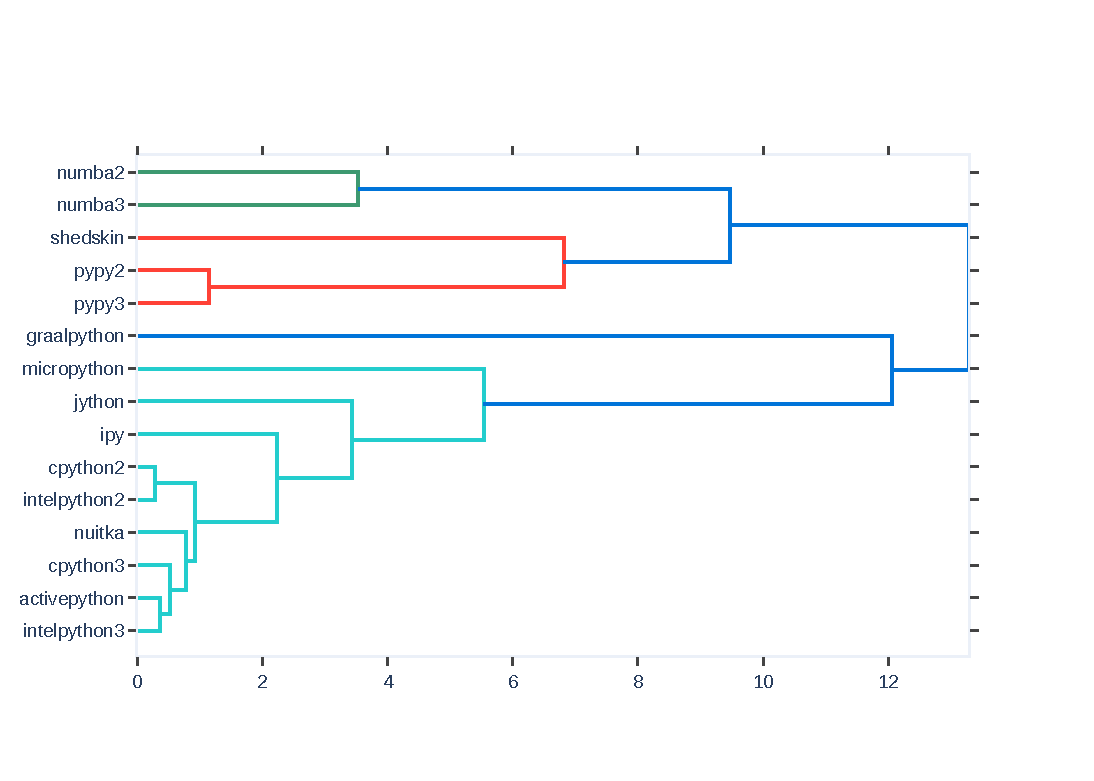
\includegraphics[width=\linewidth]{imgs/dendogram_interpreters}
      \caption{Dendogram of the different implementations}
      \label{fig:dendogram}
\end{figure}

Except GraalPython, one can notice 3 main clusters.
The first cluster contains the reference implementations (CPython2 and CPython3) and the implementations that are based on interpreters (IronPython, IntelPython, ActivePython, Jython, and Nuitka).
Moreover, each implementation is the closest to its reference Python version.
The interpreters that are based on other virtual machines, such as Jython with JVM and IronPython with .NET, behave slightly differently from the reference implementation.
As for the MicroPython, It is the furthest from the references due to his behavior toward exceptions.
The second cluster groups the interpreter implementations that are based on a JIT compiler (PyPy2 and PyPy3).
Closer to them we find Shedskin, which is a translator that converts the Python code into C++ code to be later compiled into binary code.
Table~\ref{table:manwithyu} shows that this cluster is by far the most energy-efficient one.
While Numba2 and Numba3 are also JIT libraries, they differ from PyPy due to their manual optimization.
Unlike PyPy, which will decide by itself which part of Python to optimize.
In Numba, the developer must target the portion of the code that will be passed to JIT, while the rest of the code will be executed by the regular interpreter (aka CPython).

\paragraph{Remark:}
Because GraalPython was still in its early stages, some techniques required an abnormally lengthy time, affecting the clustering algorithm.

To help practitioners to choose the best implementation for their use case, we have created a chart that describes the behavior of each implementation toward a specific aspect of programming.
Figure~\ref{fig:tommi_all} introduces a radar plot for all the implementations that have been used in this experimentation.

\begin{figure}[!htb]
      \centering
      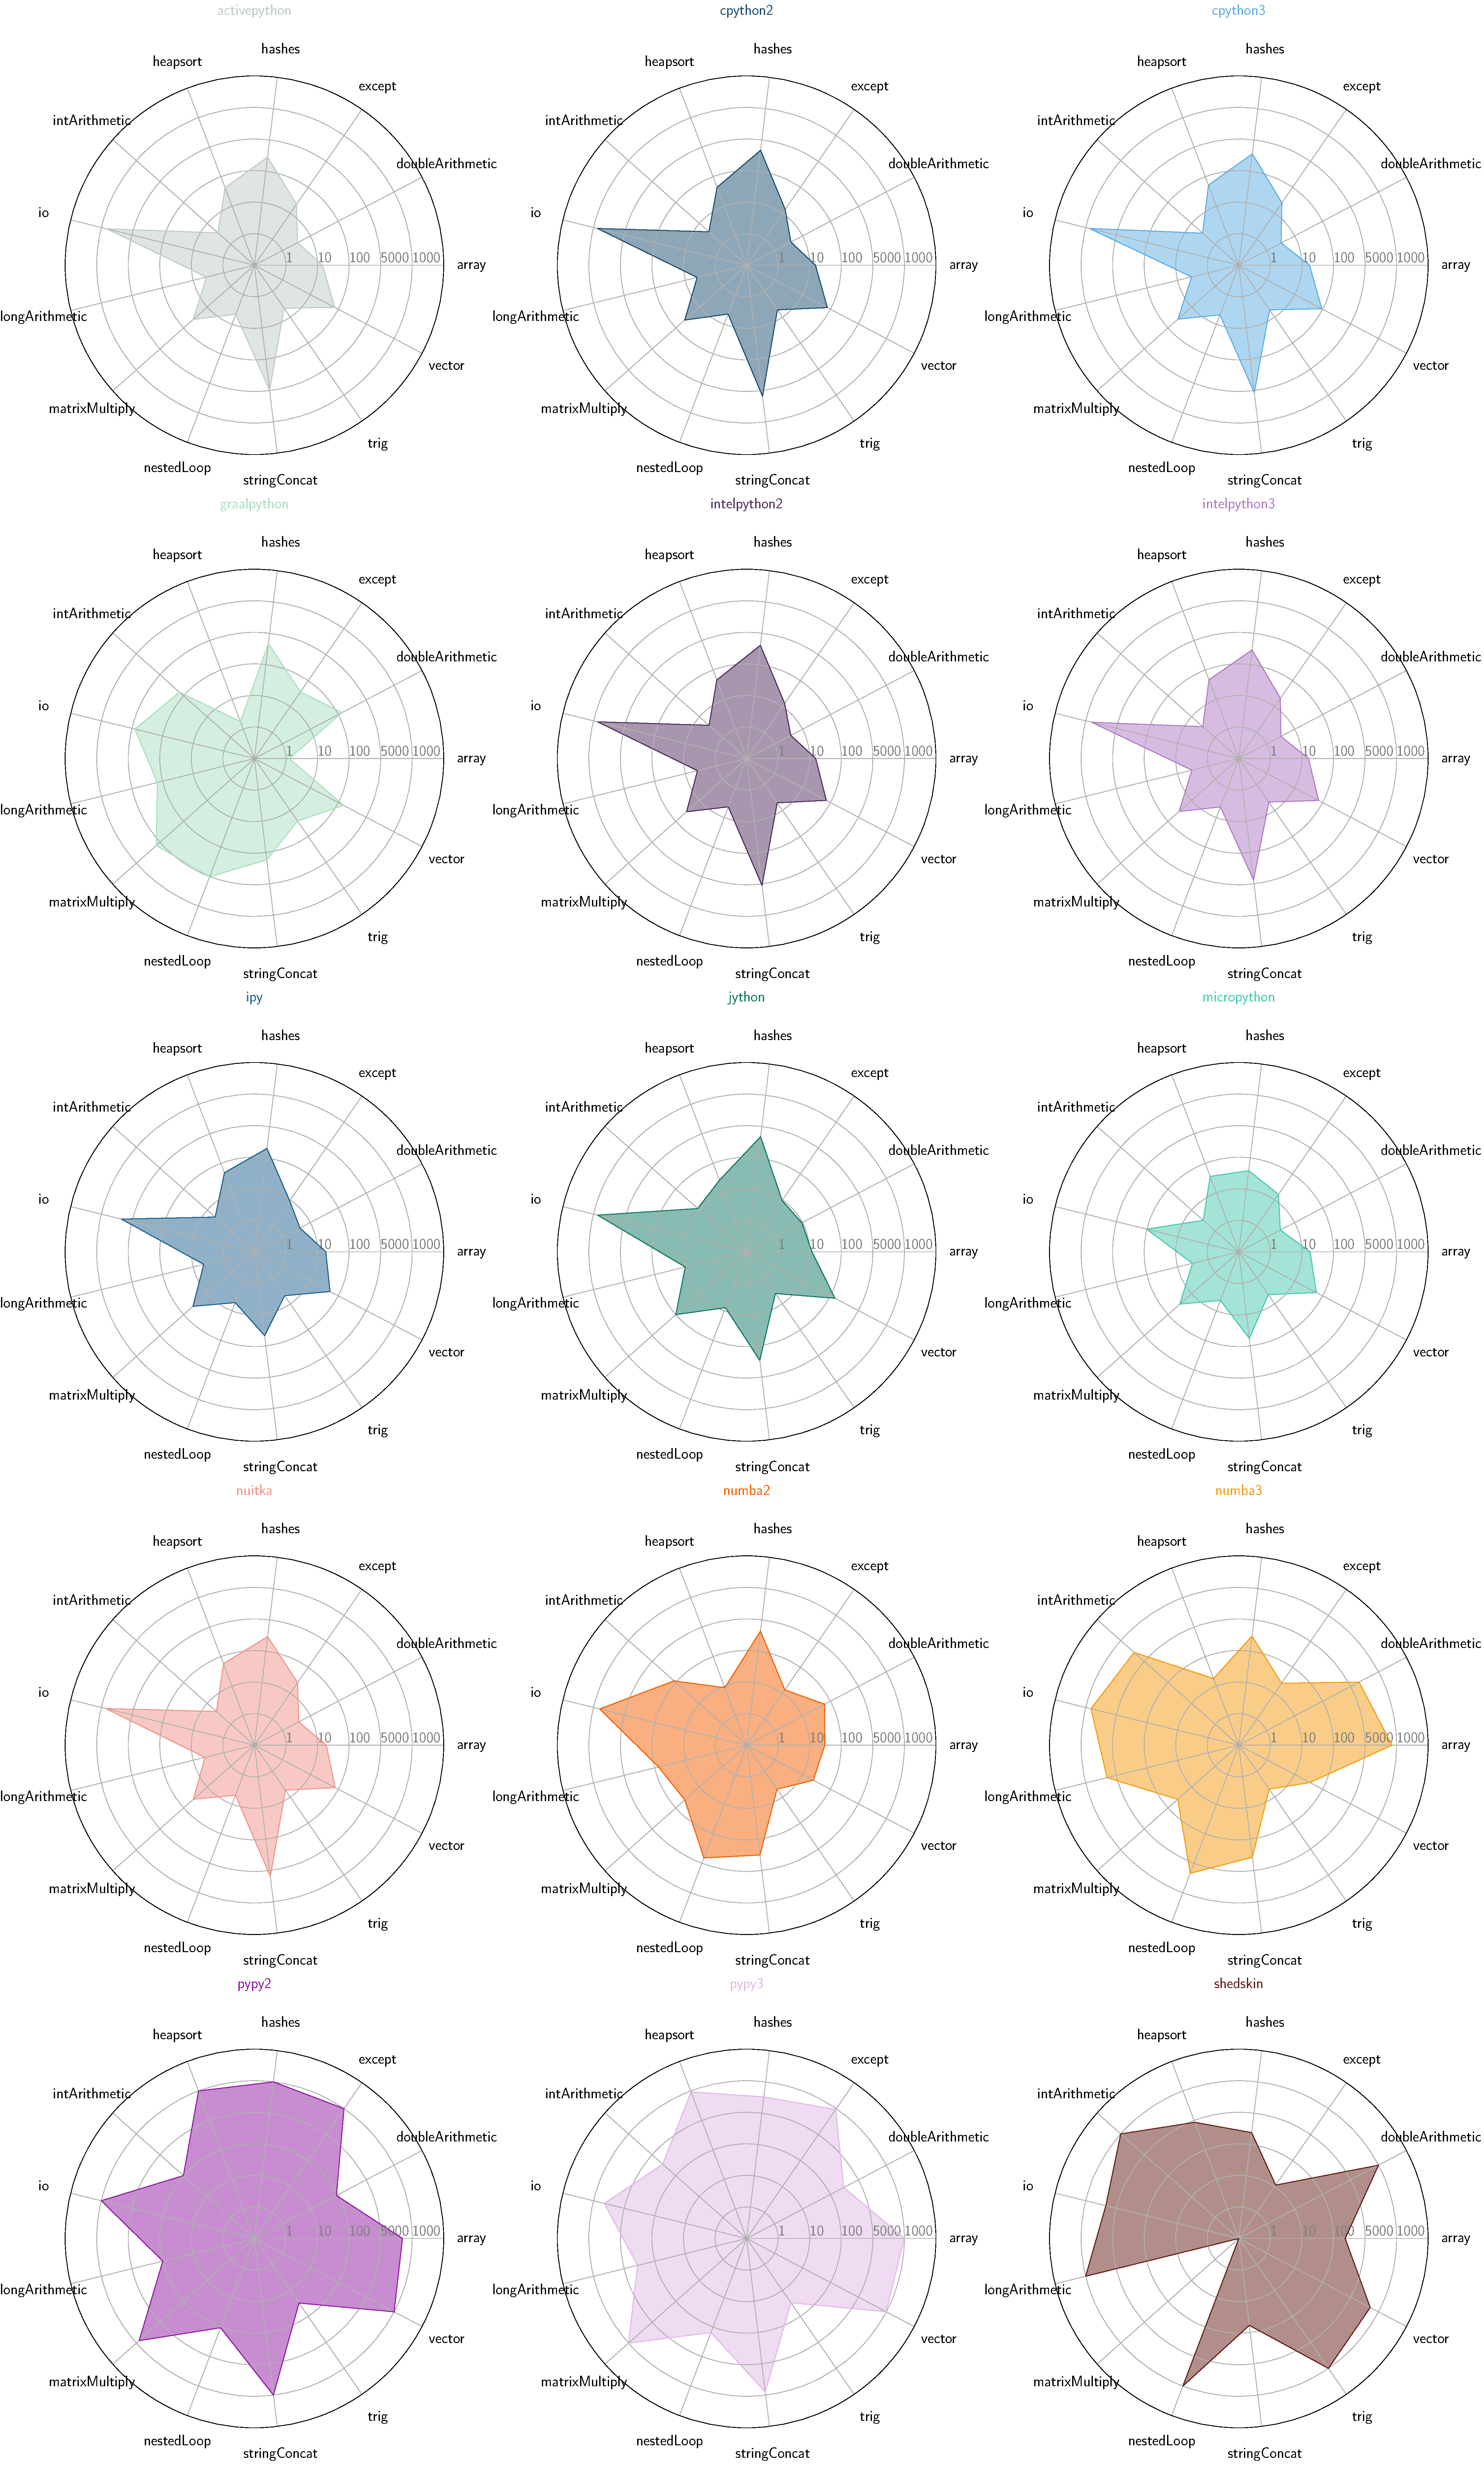
\includegraphics[width=1.0\linewidth]{imgs/alltomti_performance}
      \caption{Different interpreter's energy scores.}
      \label{fig:tommi_all}
\end{figure}

This graph summarizes each implementation energy score when executing our benchmark.
The lower the energy consumption, the higher the score.
We adopted a logarithmic scale to help the practitioners to compare numerous implementations due to the large differences between them.


As one can notice in Figure~\ref{fig:tommi_all}, there is no evolution between CPython2 and CPython3.
Moreover, IntelPython, and ActivePython all behave similarly to the reference implementation.
Therefore, one can conclude that the work done on those interpreters is primarily to improve a specific purpose and not the core interpreter.
ActivePython states that their version is focused on security and prepackaged libraries, which explains why it is slower than other versions due to the addition of this security support.\footnote{\url{https://www.activestate.com/solutions/why-activestate/}}
As for IntelPython, it is designed for machine learning.
Unfortunately, the \textsc{Tommti} benchmark is geared for general-purpose programming.
Despite the fact that Nuitka is a compiler, there was no discernible difference in energy consumption.
It was even more similar to the reference Python implementation than other interpreters.
However, if we look at the Nuitka techniques, we can see that they simply encapsulate the Python code with an interpreter into a single executable.
Finally, Shedskin reports on the best energy consumption pattern when it comes to arithmetic operations.
One can conclude it is due to the fact of the native type of the variables, unlike in the JIT, where they are treated as objects in the beginning.

Regarding the other VM-based interpereters, Jython and Ipy lacked in terms of energy optimization, which expected as they were at the beginning of the development stage and the main purpose of such implementation is to link the bytecode generated by Jython and IronPython with their respective virtual machines.

Unlike the previous interpeters, GraalPython exhibits a certain promise when it comes to complex algorithms (nested loops in particular).
% Finally, MicroPython is dedicated to embedded systems, so claiming it is a powerful CPU machine will be misleading.

% When it comes to  the input outputs operations , 
% when it came to input/output manupulation. Except for Jython,most of the interpreters behaved similarly . Because these operations are more dependent on the hardware than the interpreter.


% However, Jython is the only implementation that has a significant difference in energy consumption. This is due to the fact that Jython is based on the JVM, which is a virtual machine that is designed to run Java bytecode. Therefore, the energy consumption of the input/output operations is not the same as the other implementations.


% \begin{figure}
%       \centering
%       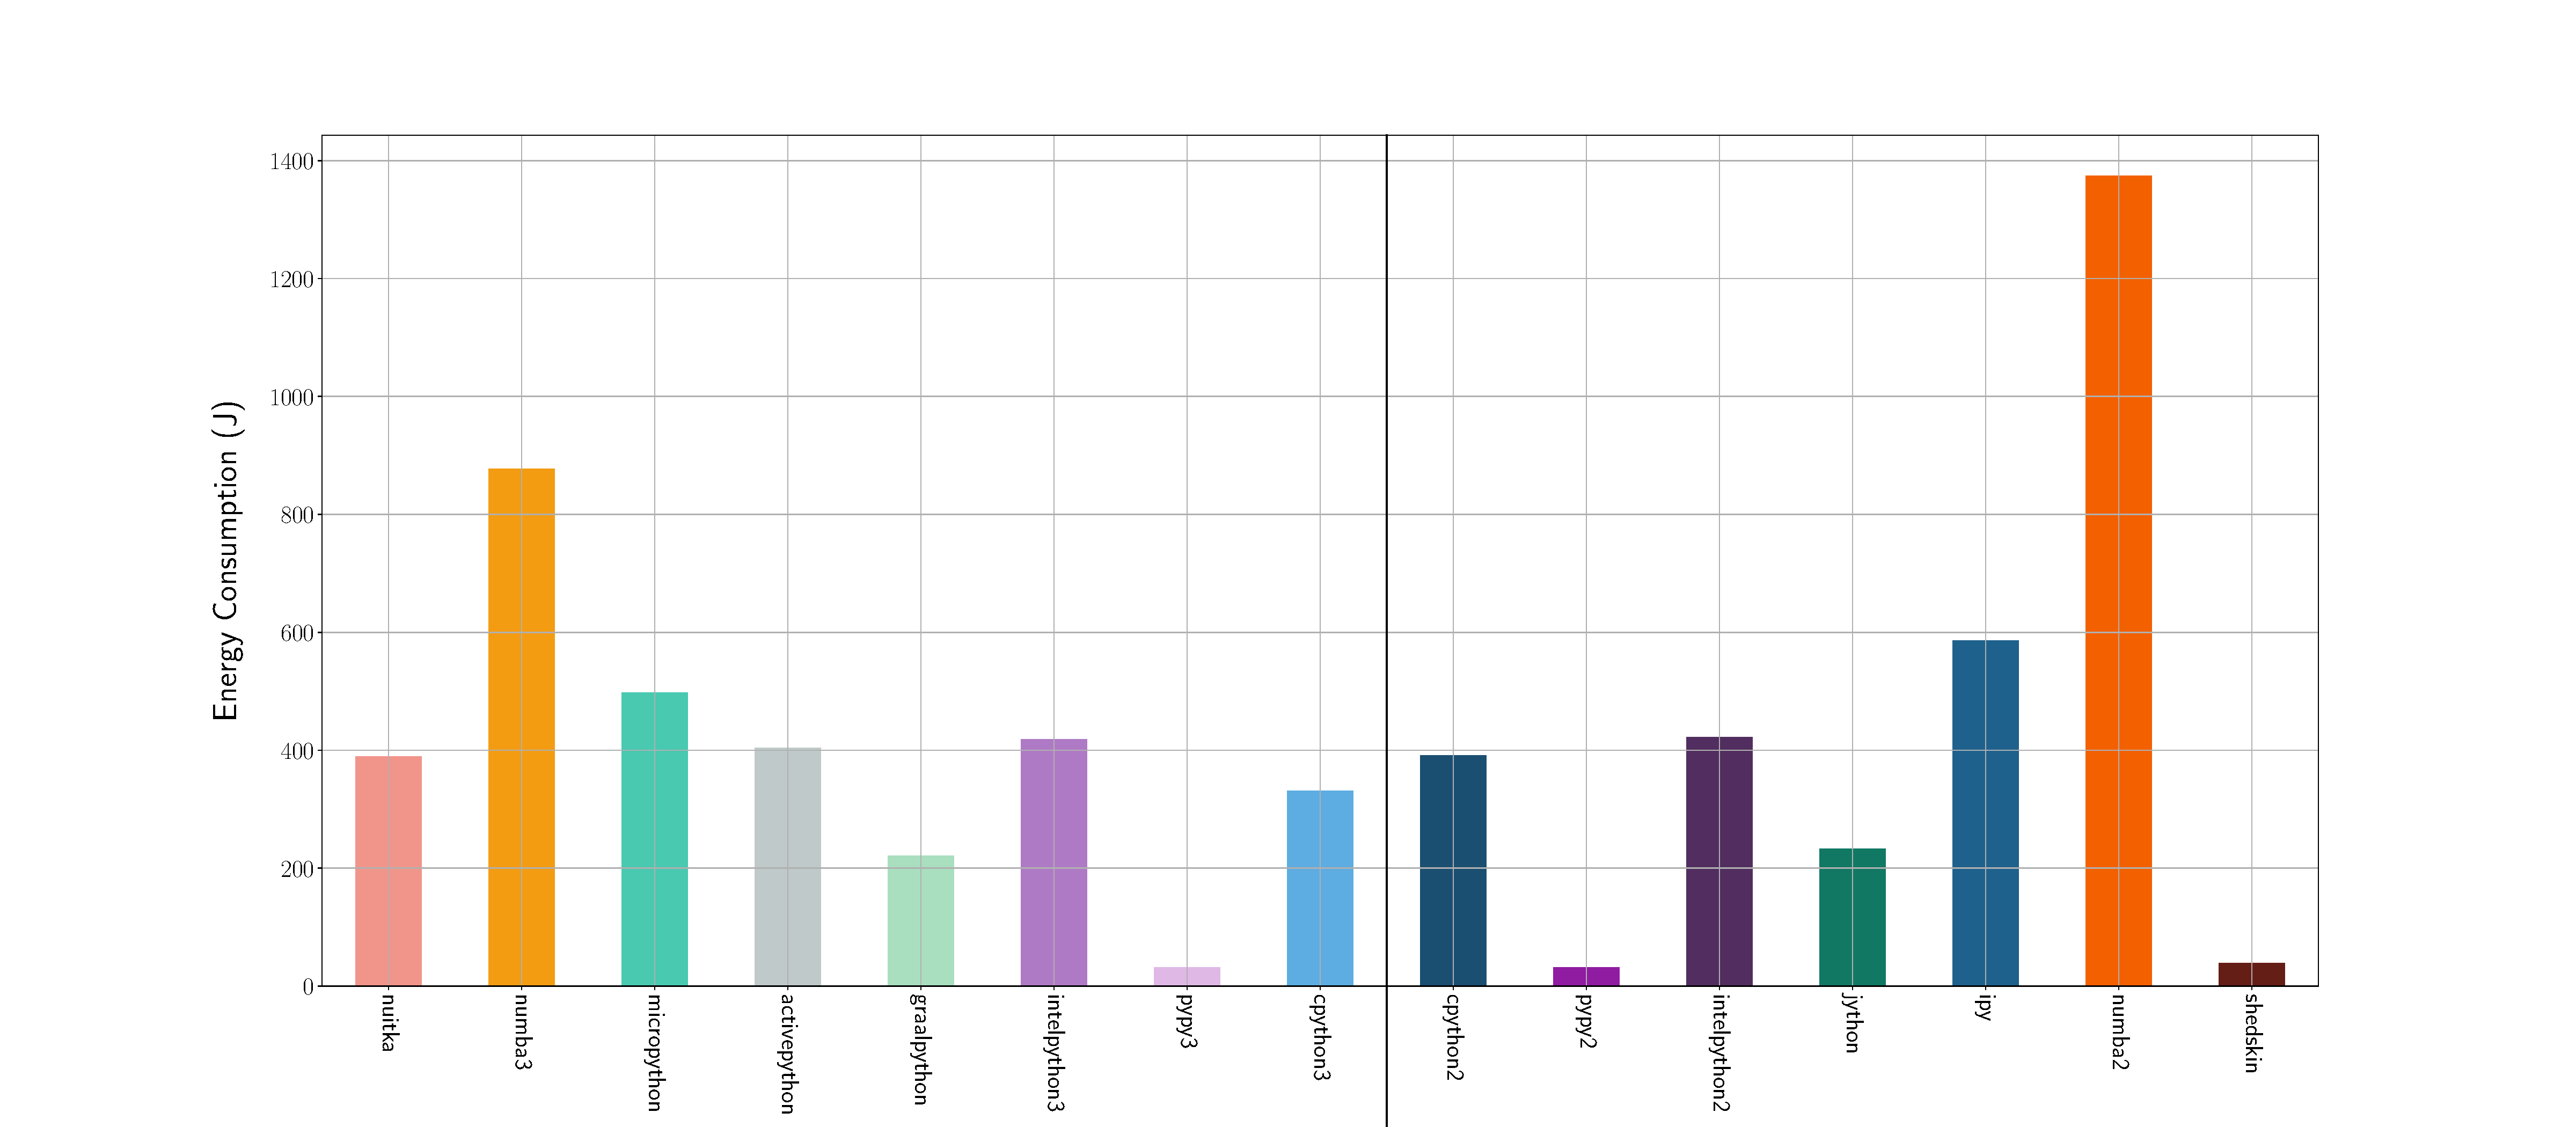
\includegraphics[width=\linewidth]{imgs/bar_plot_tommtivector}
%       \caption{Average energy consumption of different python implementaions for vector treatement}
%       \label{fig:bar_tommti_vector}
%   \end{figure}
% as usual there is  correlaction between DRAM and CPU so no need to classify based on DRAM + the DRAM consumes less 10\% of the  energy compared to the CPU

% then we use the multiparameter optimization , howerver we stop in the phase where we calculate the score
% because we dont know the weight of each parameter ( of tommti microbenchmark) and instead of doing the sum with the coefissients we use the radar plot to let the reader decide which one is the most suitable for his usage. howerver since the differences are gigantics we change the scale to logarithmic to be easier for the eye to read

% \begin{figure}
%     \centering
%     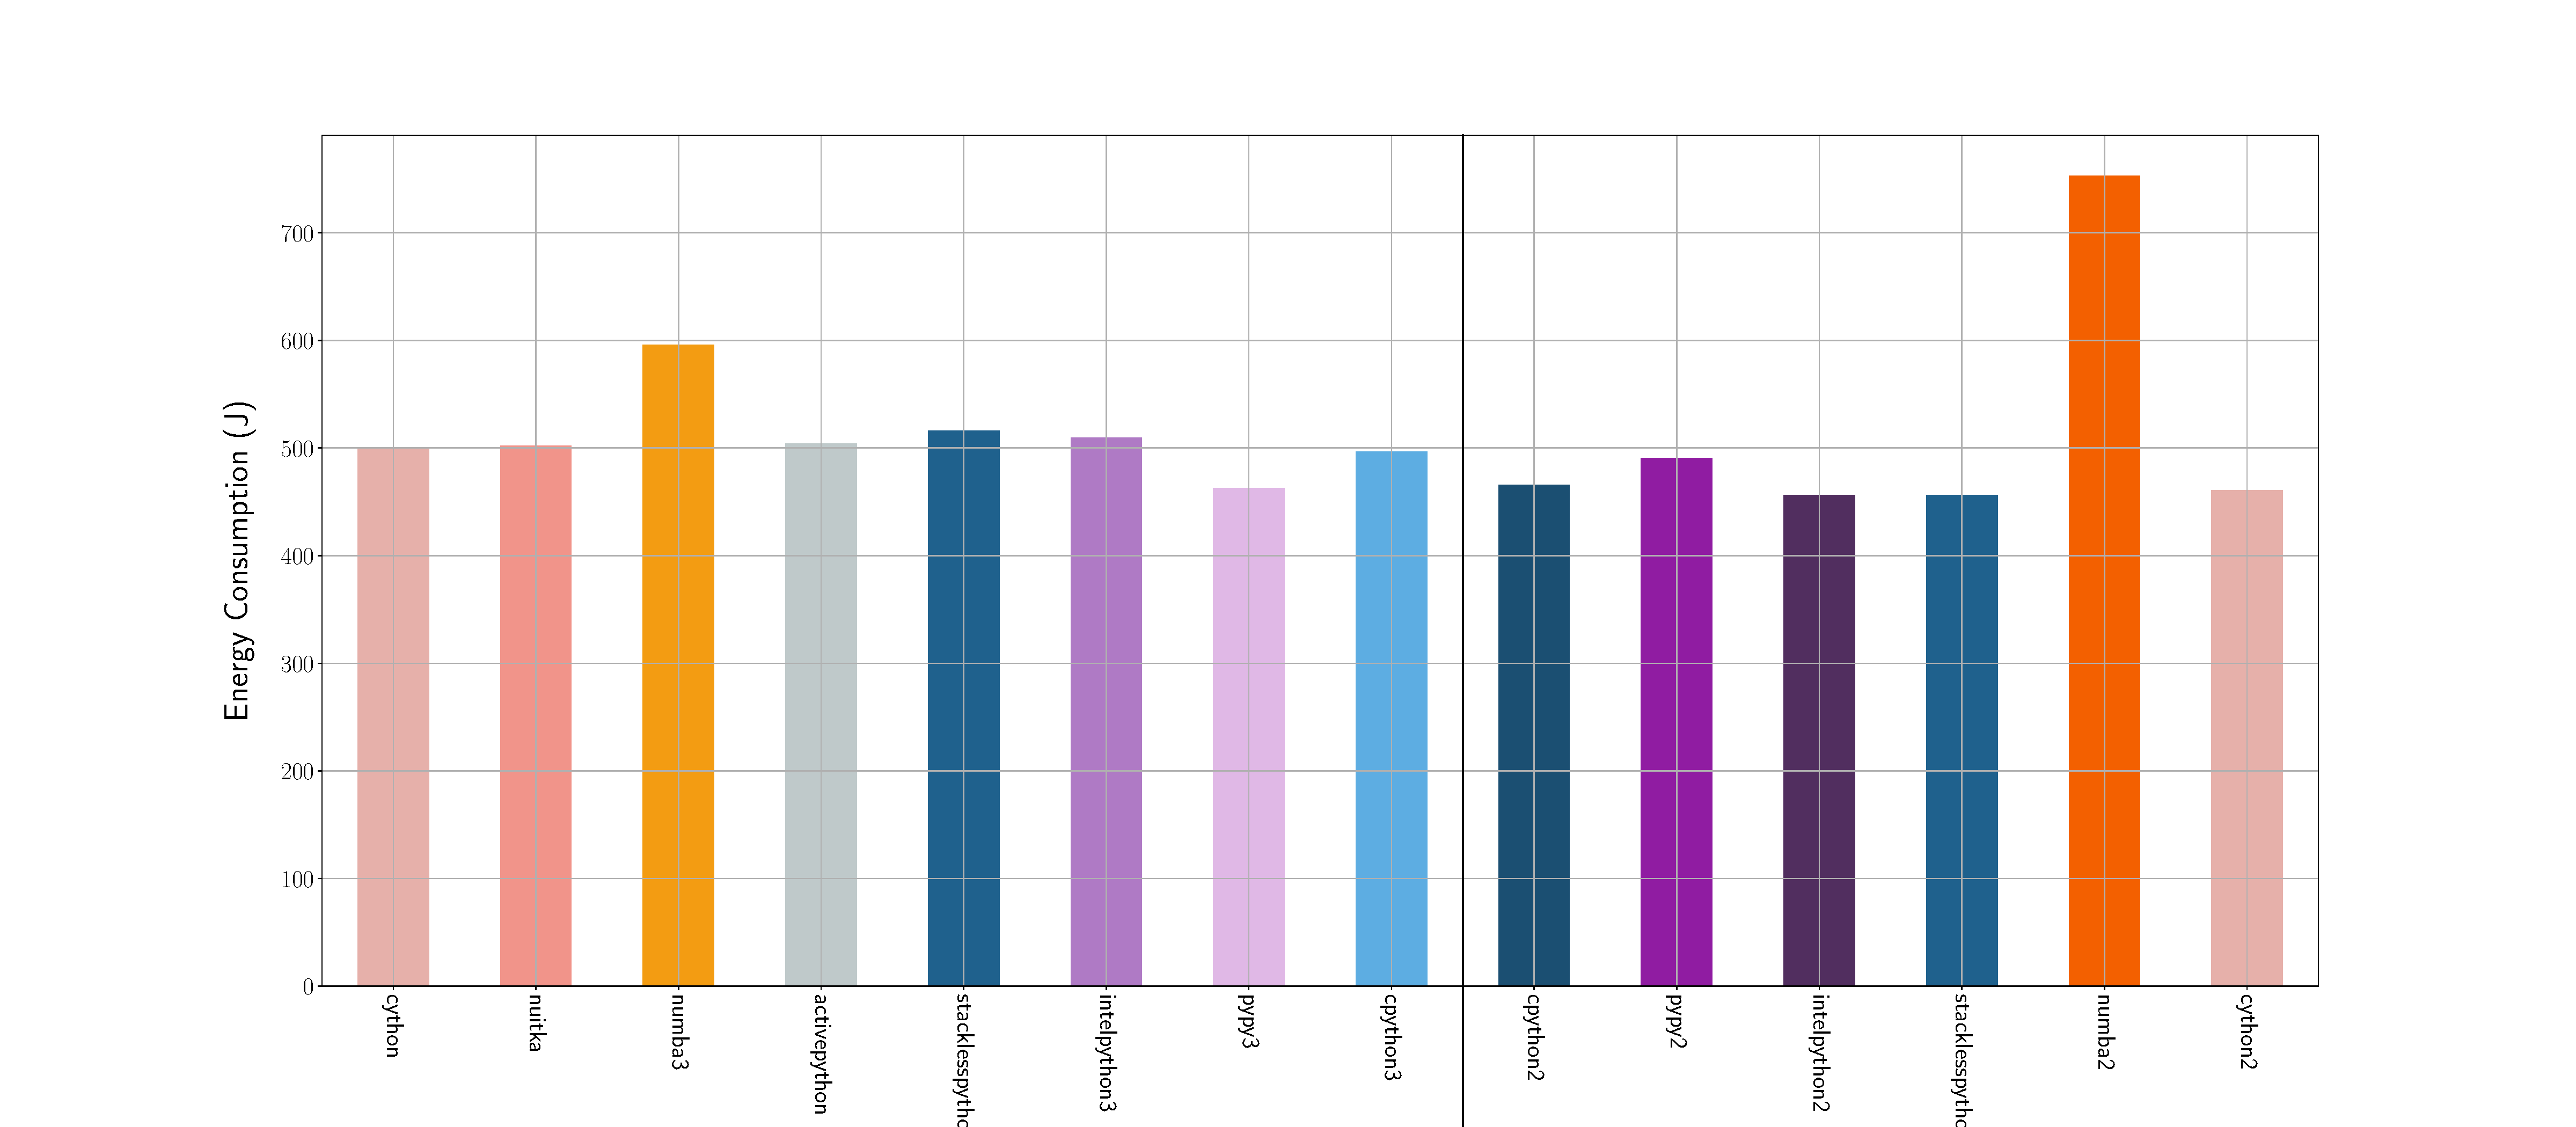
\includegraphics[width=\linewidth]{imgs/barplot_binarry_tree}
%     \caption{energy behaviour of different python implementations for the binarry Tree benchmark}
%     \label{fig:binarrytree}
% \end{figure}

% \begin{table*}

    \caption{Energy consumption python environment}
    \label{table:GC}
    \resizebox*{\linewidth}{!}{
        \begin{tabular}{l|rr|rr|rr|rr|rr|rr}
            \toprule

            Implementation & \multicolumn{2}{c}{array} & \multicolumn{2}{c}{intArithmetic} & \multicolumn{2}{c}{doubleArithmetic} & \multicolumn{2}{c}{hashes} & \multicolumn{2}{c}{heapsort} & \multicolumn{2}{c}{trig}                                                                                         \\
            \midrule

                           & energy (J)                & \em p-values                      & energy (J)                           & \em p-values               & energy (J)                   & \em p-values             & energy (J)     & \em p-values & energy (J) & \em p-values & energy (J) & \em p-values \\
            activepython   & 4e02                      & 0.0079                            & 6.9e02                               & 0.0022                     & 6.6e02                       & 0.0043                   & 9.7e02         & 0.0079       & 2.9e02     & 0.0079       & 5.1e02     & 0.0079       \\
            cpython2       & 3.4e02                    & 0.0079                            & 5.6e02                               & 0.0022                     & 5.5e02                       & 0.0043                   & 6.5e02         & 0.0079       & 2.9e02     & 0.0079       & 4.1e02     & 0.0079       \\
            cpython3       & 3.2e02                    & 0.0079                            & 7.4e02                               & 0.0022                     & 7.3e02                       & 0.0043                   & 7.9e02         & 0.0079       & 2.4e02     & 0.0079       & 4.1e02     & 0.0079       \\
            graalpython    & 1.2e05                    & 0.0079                            & 24                                   & 0.0022                     & 24                           & 0.0043                   & 6.4e02         & 0.0079       & 1.3e05     & 0.0079       & 72         & 0.0079       \\
            intelpython2   & 3.7e02                    & 0.0079                            & 5.9e02                               & 0.0022                     & 5.6e02                       & 0.0043                   & 7.1e02         & 0.0079       & 2.7e02     & 0.0079       & 4.2e02     & 0.0079       \\
            intelpython3   & 3.5e02                    & 0.0079                            & 7.7e02                               & 0.0022                     & 7.6e02                       & 0.0043                   & 9.4e02         & 0.0079       & 2.6e02     & 0.0079       & 4.8e02     & 0.0079       \\
            ipy            & 3e02                      & 0.0079                            & 4.4e02                               & 0.0022                     & 4.7e02                       & 0.0079                   & 1.3e03         & 0.0079       & 2.6e02     & 0.0079       & 4.5e02     & 0.0079       \\
            jython         & 5.2e02                    & 0.0079                            & 1.3e02                               & 0.0022                     & 1.6e02                       & 0.0043                   & 6.4e02         & 0.0079       & 4.6e02     & 0.0079       & 6.2e02     & 0.0079       \\
            micropython    & 3.1e02                    & 0.0079                            & 8.2e02                               & 0.0022                     & 8.4e02                       & 0.0079                   & 9.5e03         & 0.0079       & 3.4e02     & 0.0079       & 5.3e02     & 0.0079       \\
            nuitka         & 2.9e02                    & 0.0079                            & 5.4e02                               & 0.0022                     & 5.5e02                       & 0.0079                   & 9.5e02         & 0.0079       & 2.2e02     & 0.0079       & 3.9e02     & 0.0079       \\
            numba2         & 1.9e02                    & 0.0079                            & 27                                   & 0.0022                     & 36                           & 0.0079                   & 6.8e02         & 0.0079       & 2.1e03     & 0.0079       & 4.4e02     & 0.0079       \\
            numba3         & \best{11}                 & \best{best}                       & 10                                   & 0.0022                     & 10                           & 0.0079                   & 9.1e02         & 0.0079       & 7.2e02     & 0.0079       & 4.5e02     & 0.0079       \\
            pypy2          & 16                        & \same{0.15}                       & 29                                   & 0.0022                     & 30                           & 0.0043                   & \best{ 1.1e02} & \best{best}  & \best{20}  & \best{best}  & 64         & 0.0079       \\
            pypy3          & 13                        & \same{0.15}                       & 17                                   & 0.0022                     & 18                           & 0.0079                   & 1.9e02         & 0.0079       & \best{20}  & 0.31         & 65         & 0.0079       \\
            shedskin       & 47                        & 0.0079                            & \best{7.4}                           & \best{best}                & \best{7.3 }                  & \best{best}              & 1.1e03         & 0.0079       & 44         & 0.0079       & \best{7.7} & \best{best}  \\
            \bottomrule
        \end{tabular}

    }
    \vfill
    \resizebox*{\linewidth}{!}{
        \begin{tabular}{l|rr|rr|rr|rr|rr|rr}

            Implementation & \multicolumn{2}{c}{longArithmetic} & \multicolumn{2}{c}{matrixMultiply} & \multicolumn{2}{c}{io} & \multicolumn{2}{c}{stringConcat} & \multicolumn{2}{c}{nestedLoop} & \multicolumn{2}{c}{except}                                                                                     \\
            \midrule
                           & energy (J)                         & \em p-values                       & energy (J)             & \em p-values                     & energy (J)                     & \em p-values               & energy (J) & \em p-values & energy (J) & \em p-values & energy (J) & \em p-values \\
            activepython   & 6.7e02                             & 0.0079                             & 4.3e02                 & 0.0079                           & 2.1e02                         & 0.0079                     & 14         & 0.0079       & 4.1e02     & 0.0079       & 2.6e02     & 0.0079       \\
            cpython2       & 5.5e02                             & 0.0079                             & 4e02                   & 0.0079                           & 2e02                           & 0.0079                     & 12         & 0.0079       & 4.2e02     & 0.0079       & 4.3e02     & 0.0079       \\
            cpython3       & 7.4e02                             & 0.0079                             & 4.4e02                 & 0.0079                           & 2e02                           & 0.0079                     & 13         & 0.0079       & 3.8e02     & 0.0079       & 2.3e02     & 0.0079       \\
            graalpython    & 24                                 & 0.0079                             & 45                     & 0.0079                           & 7.5e02                         & 0.0079                     & 26         & 0.0079       & 12         & 0.0079       & 1.6e02     & 0.0079       \\
            intelpython2   & 5.7e02                             & 0.0079                             & 4.8e02                 & 0.0079                           & 2e02                           & 0.0079                     & 13         & 0.0079       & 4.4e02     & 0.0079       & 4.6e02     & 0.0079       \\
            intelpython3   & 7.7e02                             & 0.0079                             & 5e02                   & 0.0079                           & 2.2e02                         & 0.0079                     & 14         & 0.0079       & 4.4e02     & 0.0079       & 2.7e02     & 0.0079       \\
            ipy            & 4.7e02                             & 0.0079                             & 4.1e02                 & 0.0079                           & 3.8e02                         & 0.0079                     & 49         & 0.0079       & 3.3e02     & 0.0079       & 7.2e02     & 0.0079       \\
            jython         & 1.6e02                             & 0.0079                             & 1.9e02                 & 0.0079                           & 2e02                           & 0.0079                     & 21         & 0.0079       & 1.9e02     & 0.0079       & 7.1e02     & 0.0079       \\
            micropython    & 8.3e02                             & 0.0079                             & 5.3e02                 & 0.0079                           & 5.3e03                         & 0.0079                     & 44         & 0.0079       & 4.3e02     & 0.0079       & 3.6e02     & 0.0079       \\
            nuitka         & 5.4e02                             & 0.0079                             & 4.3e02                 & 0.0079                           & 2e02                           & 0.0079                     & 12         & 0.0079       & 3.6e02     & 0.0079       & 2.2e02     & 0.0079       \\
            numba2         & 35                                 & 0.0079                             & 4e02                   & 0.0079                           & 2.2e02                         & 0.0079                     & 20         & 0.0079       & 14         & 0.0079       & 4.5e02     & 0.0079       \\
            numba3         & 11                                 & 0.0079                             & 4.2e02                 & 0.0079                           & 2.1e02                         & 0.0079                     & 19         & 0.0079       & 10         & 0.0079       & 2.4e02     & 0.0079       \\
            pypy2          & 30                                 & 0.0079                             & 24                     & 0.056                            & \best{1.7e02}                  & \best{best}                & 7.7        & \best{best}  & 27         & 0.0079       & \best{14}  & \best{best}  \\
            pypy3          & 17                                 & 0.0079                             & \best{23}              & \best{best}                      & 2.6e02                         & 0.0079                     & 8.3        & 0.69         & 23         & 0.0079       & 14         & 0.69         \\
            shedskin       & \best{7.8}                         & \best{best}                        &                        &                                  & 3.8e02                         & 0.0079                     & 44         & 0.0079       & 7.1        & \best{best}  & 5.6e02     & 0.0079       \\

            \bottomrule
        \end{tabular}
    }

\end{table*}




%% distance euclidean 
%% linkage complete Voor Hees Algorithm. 

%%%%%%%%%%%%%%%%%


% \begin{figure}
%     \centering
%     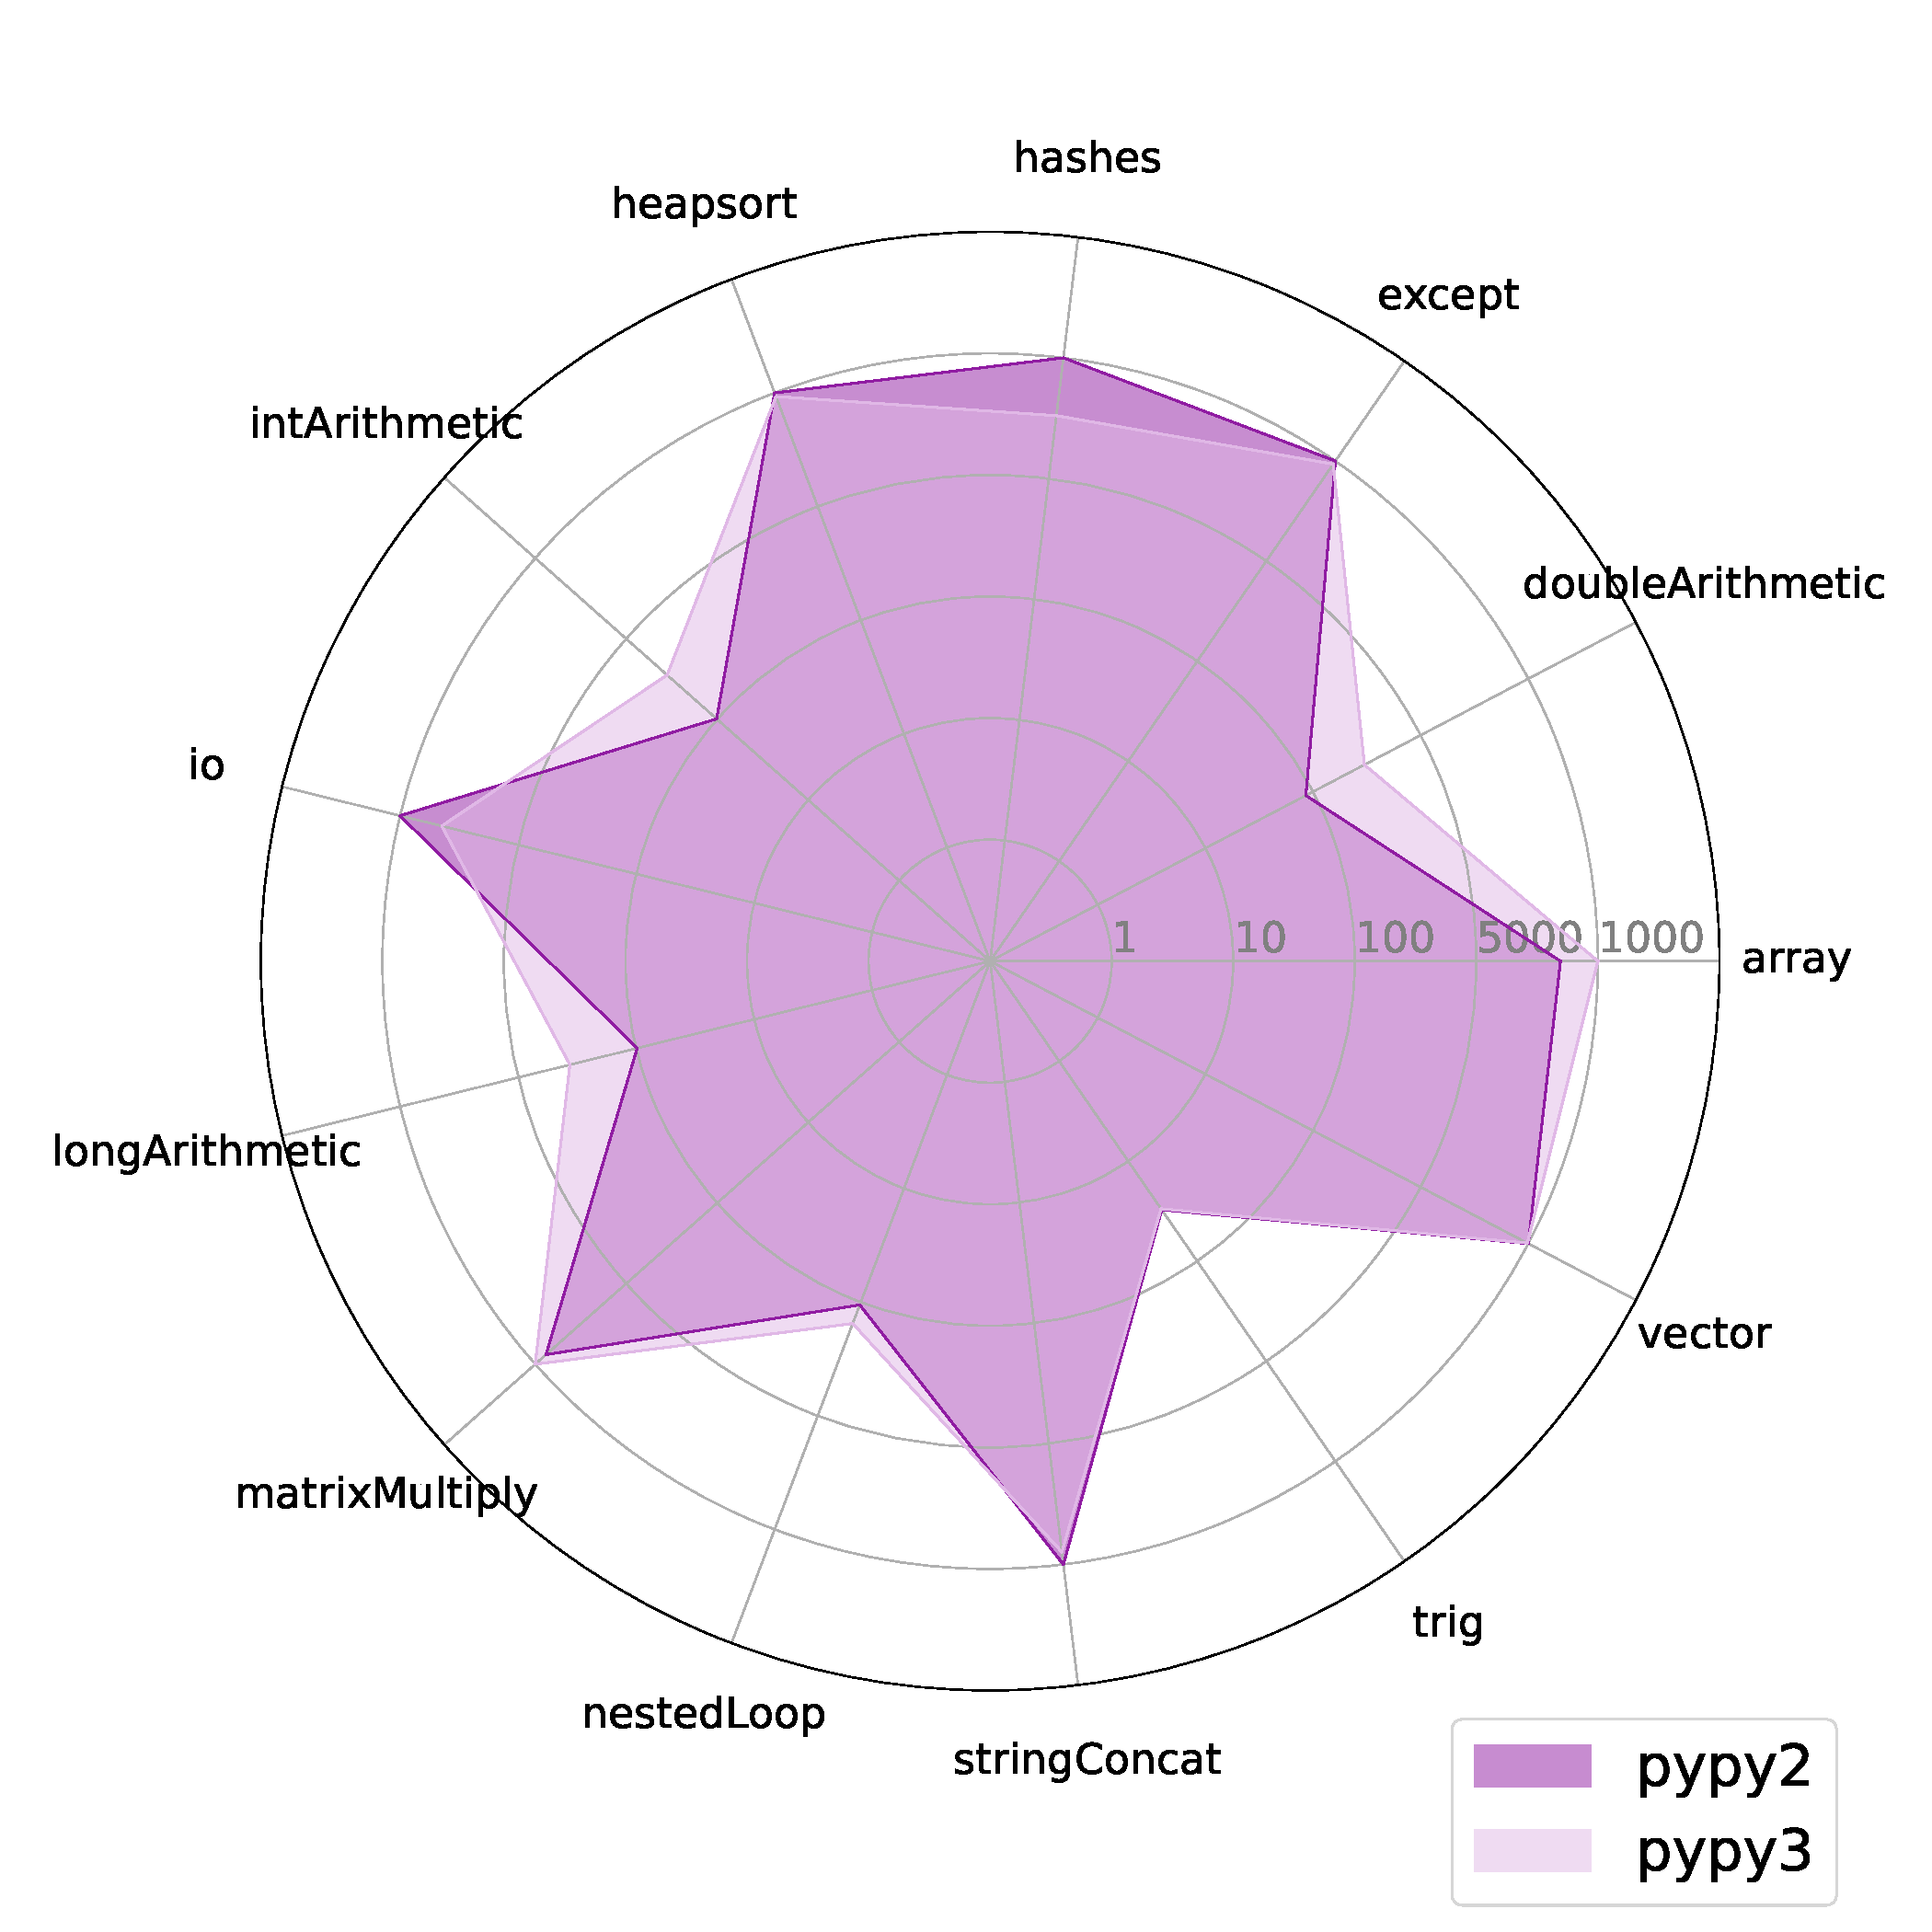
\includegraphics[width=\linewidth]{imgs/tommti_compare__pypy2_pypy3}
%     \caption{green factor of pypy }
%     \label{fig:pypy2vspypy3}
% \end{figure}

% \begin{figure}
%     \centering
%     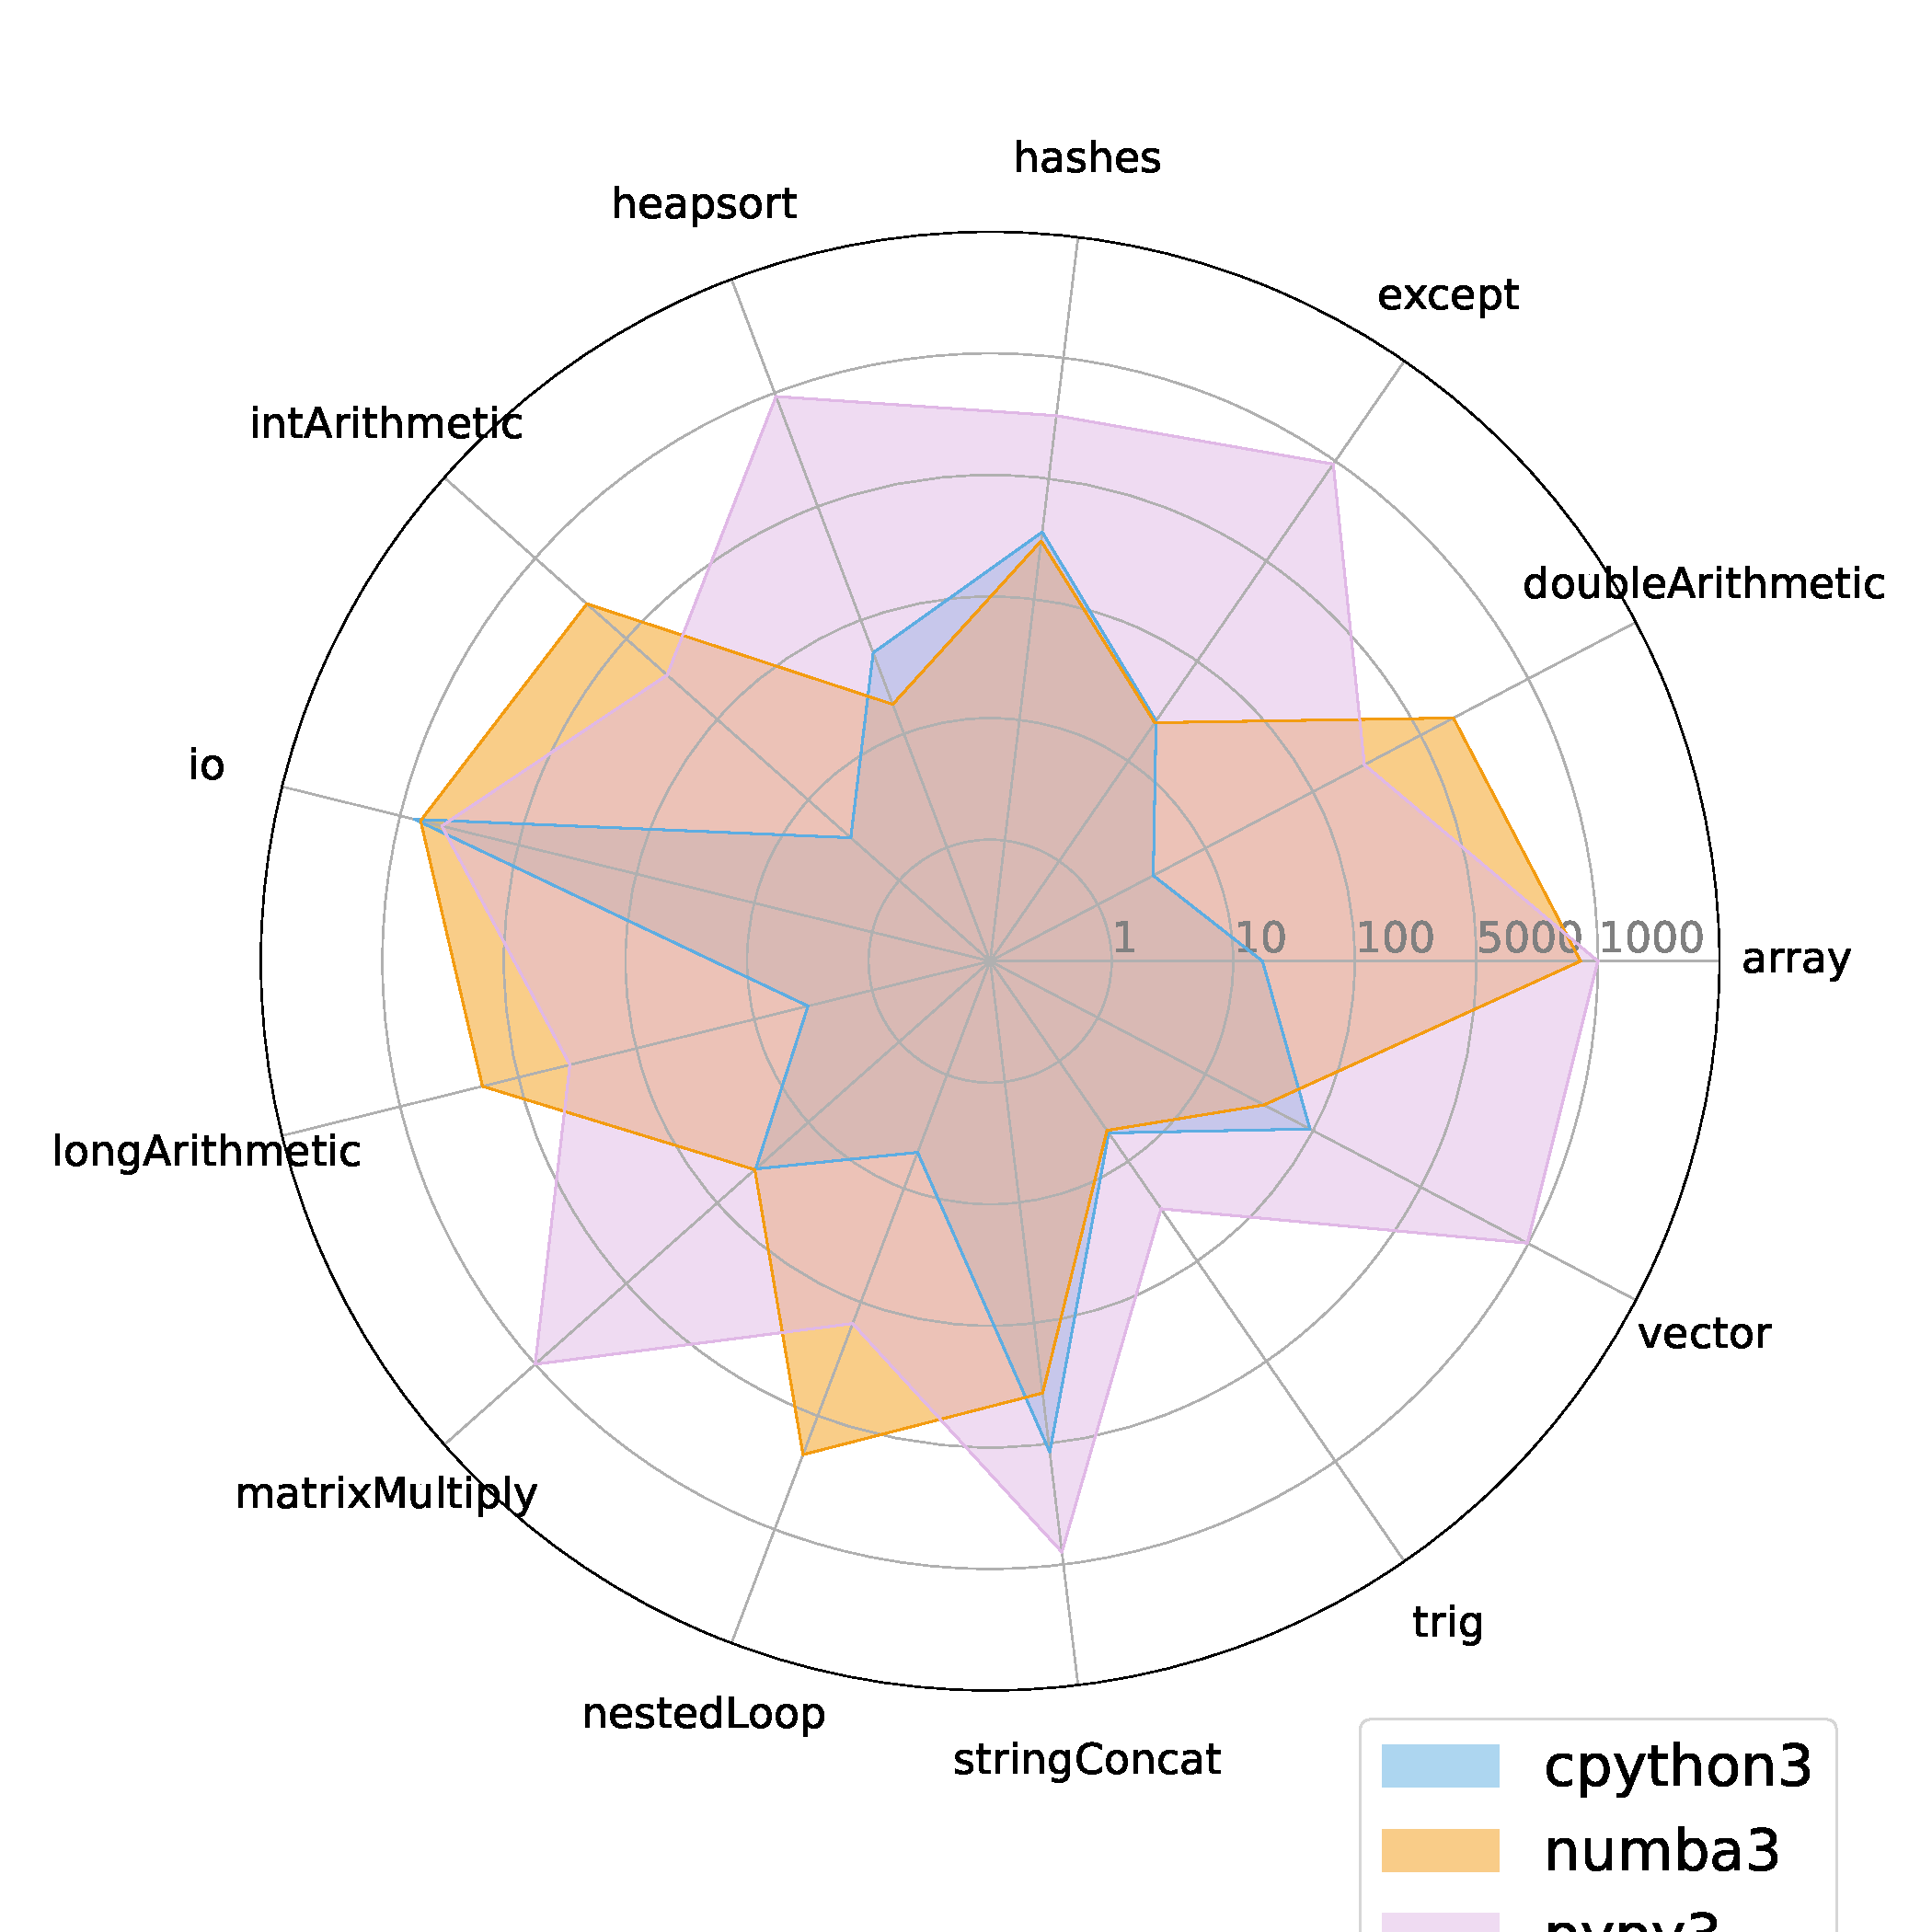
\includegraphics[width=\linewidth]{imgs/tommti_compare__cpython3_numba3_pypy3}
%     \caption{comparaison of pypy vs python vs numba }
%     \label{fig:p3}
% \end{figure}

% \begin{figure}
%     \centering
%     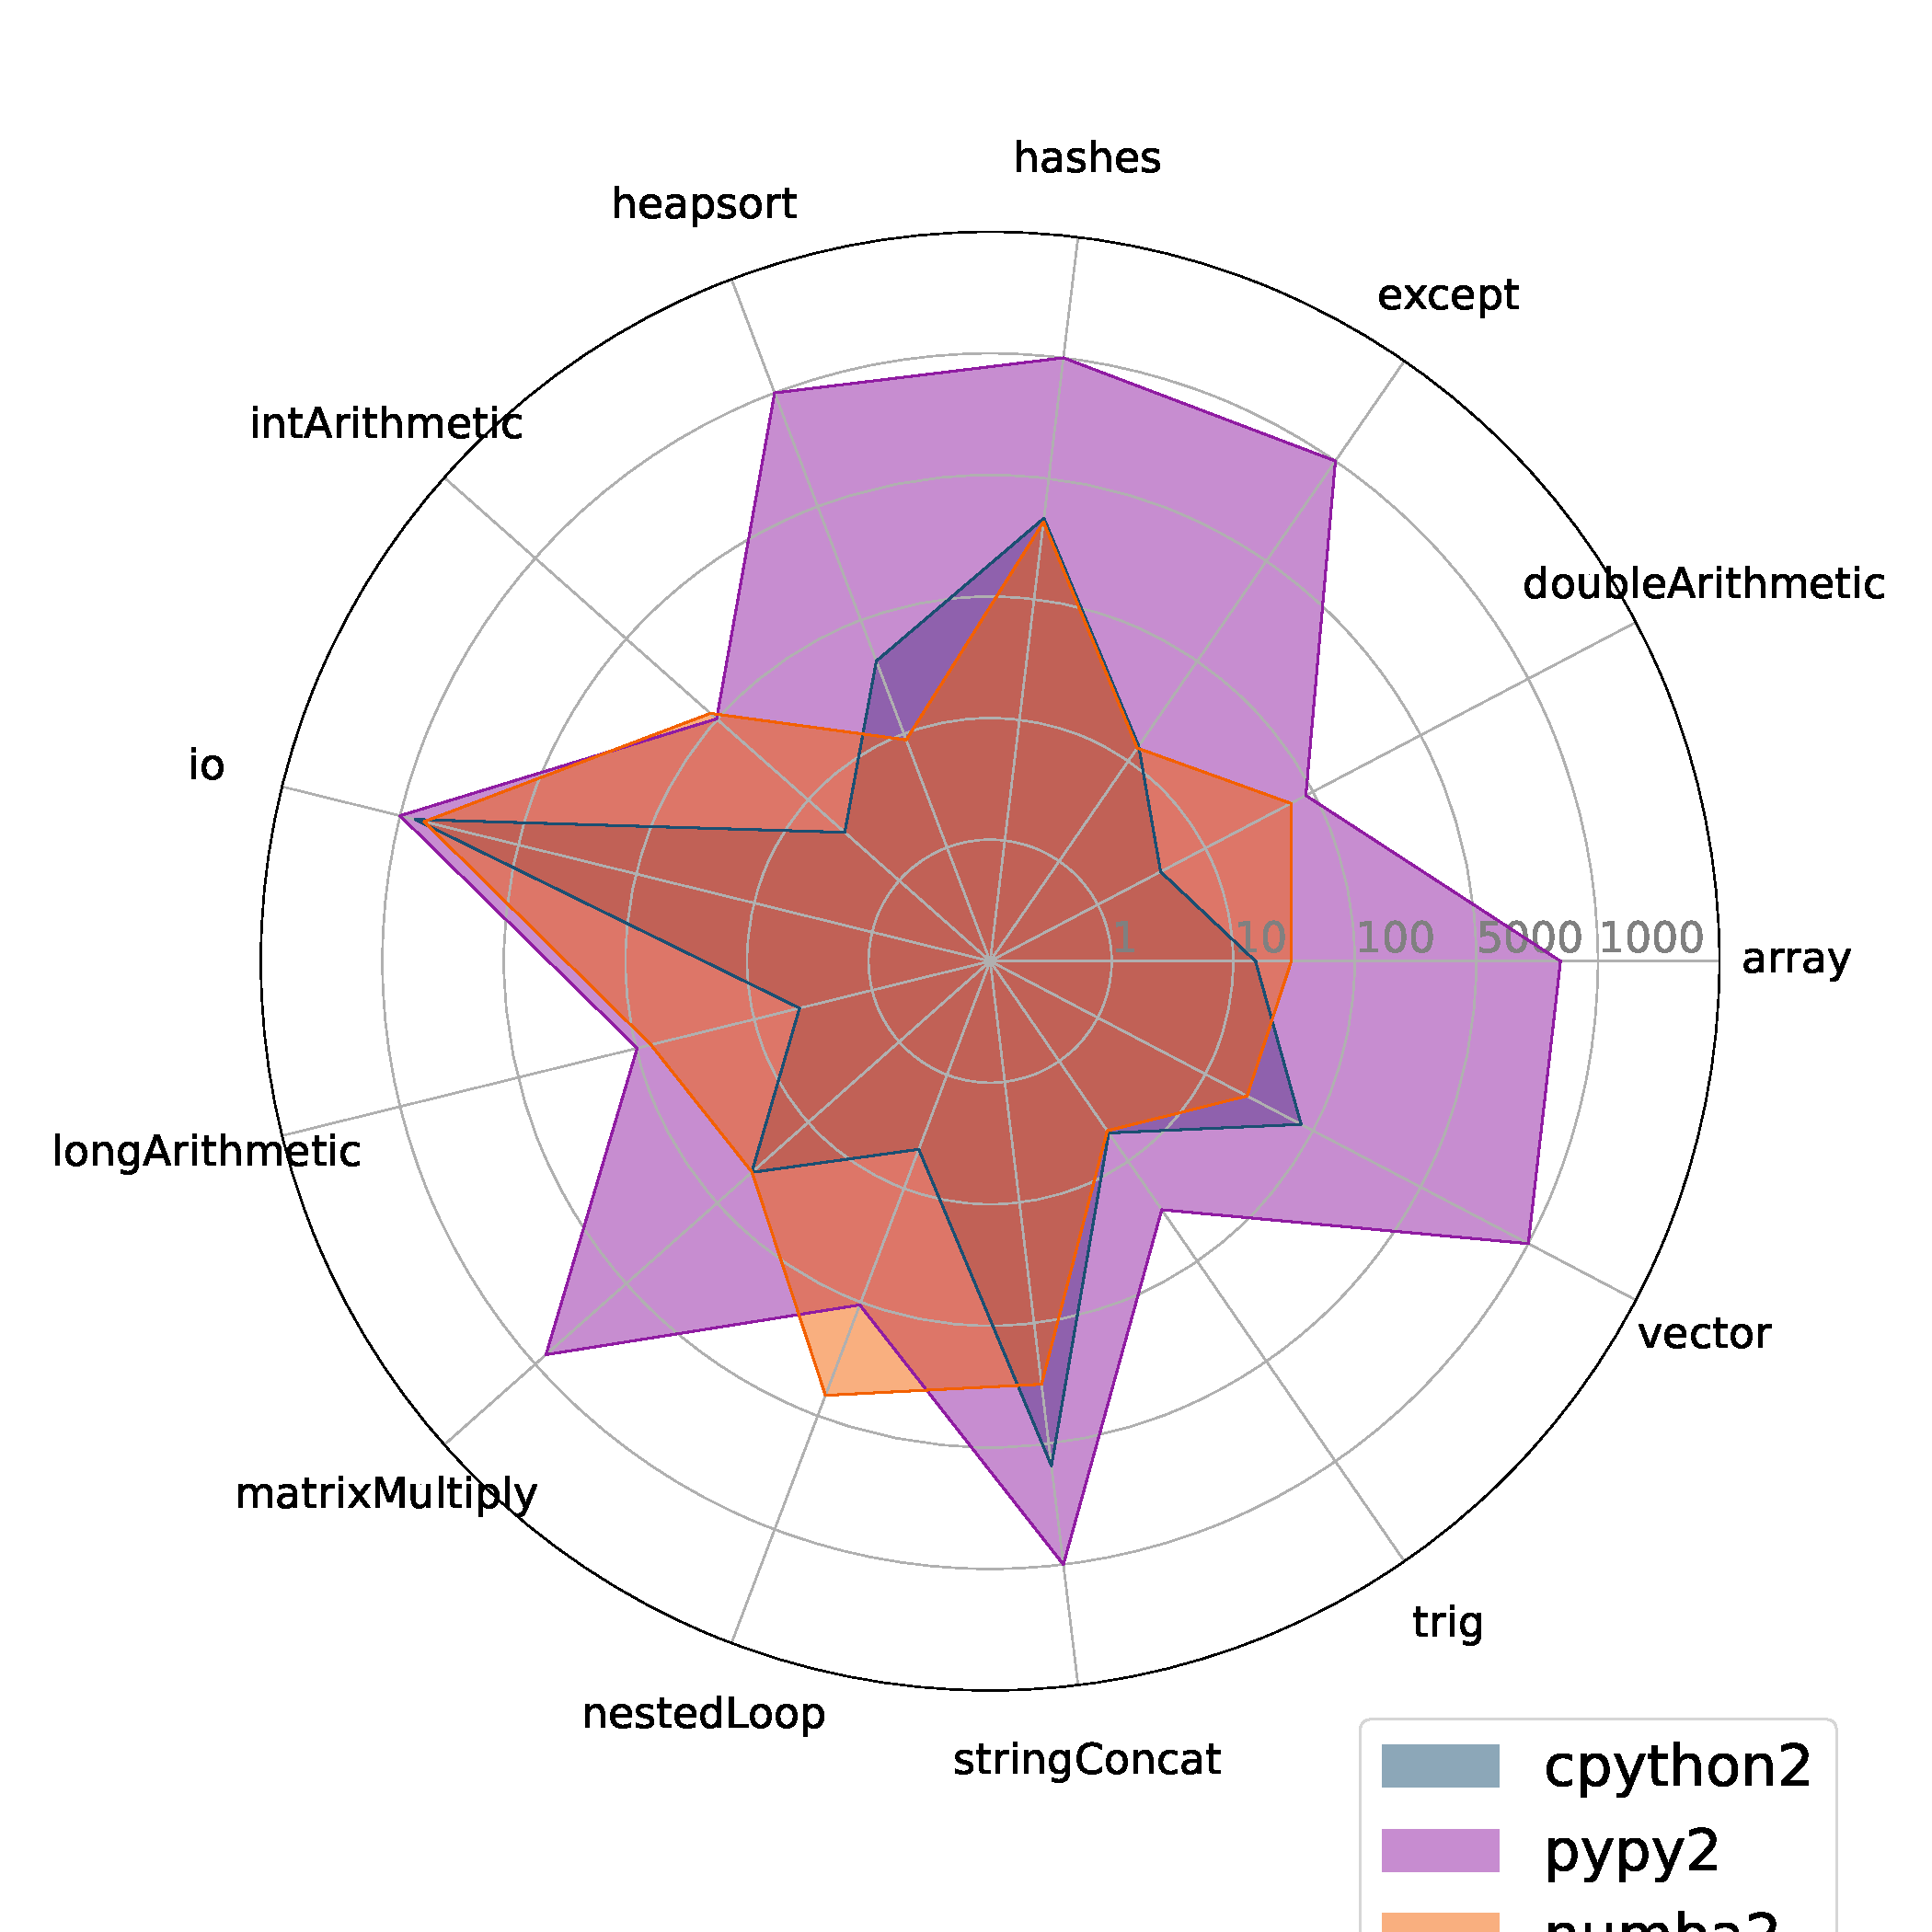
\includegraphics[width=\linewidth]{imgs/tommti_compare__cpython2_pypy2_numba2}
%     \caption{comparaison of pypy vs python vs numba }
%     \label{fig:p2}
% \end{figure}

%   this is after , when we come to the conclusion
% pypy handles exceptions very well


\subsection{Python \& Binary Operations}
The second part of this study is to look at how different Python implementations work when executing different binary operations.

\begin{figure}[!hbt]
      \small
      \center
      \begin{tabular}{|lrrrrr||r|}
            \toprule
            benchmark    & Addition & Right Rotation & Left Rotation & Or      & XOR     & Average     \\
            \midrule
            ActivePython & 676.980  & 763.208        & 651.783       & 743.016 & 728.828 & 712.76      \\
            CPython2     & 441.082  & 435.886        & 430.846       & 415.247 & 419.081 & 428.43      \\
            cpython3     & 595.209  & 685.085        & 563.839       & 657.972 & 655.560 & 531.53      \\
            \hline
            Cython       & 35.077   & 182.688        & 274.177       & 34.868  & 34.504  & 112.26      \\
            Nuitka       & 33.260   & 32.980         & 33.256        & 33.472  & 33.030  & 33.2        \\
            \hline
            Numba2       & 9.102    & 8.411          & 9.460         & 9.375   & 9.755   & \best{9.22} \\
            Numba3       & 9.566    & 10.144         & 9.219         & 9.344   & 9.665   & \best{9.59} \\
            PyPy2        & 8.456    & 7.844          & 8.286         & 8.138   & 7.952   & \best{8.13} \\
            PyPy3        & 7.552    & 8.093          & 8.108         & 8.669   & 8.623   & \best{8.21} \\
            Shedskin     & 8.024    & 8.070          & 8.399         & 8.126   & 8.277   & \best{8.18} \\
            \bottomrule
      \end{tabular}
      \caption{Energy consumption of different implementations using bit operations benchmark (in Joules).}
      \label{table:bitops}
\end{figure}


Table~\ref{table:bitops} provides a detailed report on the energy consumption of different implementations of the code.
Besides \emph{Cython}, each implementation treats the binary operation the same.
As one can see, Table~\ref{table:bitops} shows no difference in the energy consumption of those operations.
However, when it comes to Cython, the rotation operations tend to consume 5 times more energy than the other operations, and left rotations consume even more than the right ones.
The reason behind such behavior is the fact that Cython does not have a native implementation for these two operations, so it replaces them with more complex operations, which leads to an overhead of $6s$ for the right rotation and $10s$ for the left, compared to $1.5s$ for the other operations.
Therefore, it is safe to summarize all the operations into one that we call \emph{binary}.

\begin{figure}
      \centering
      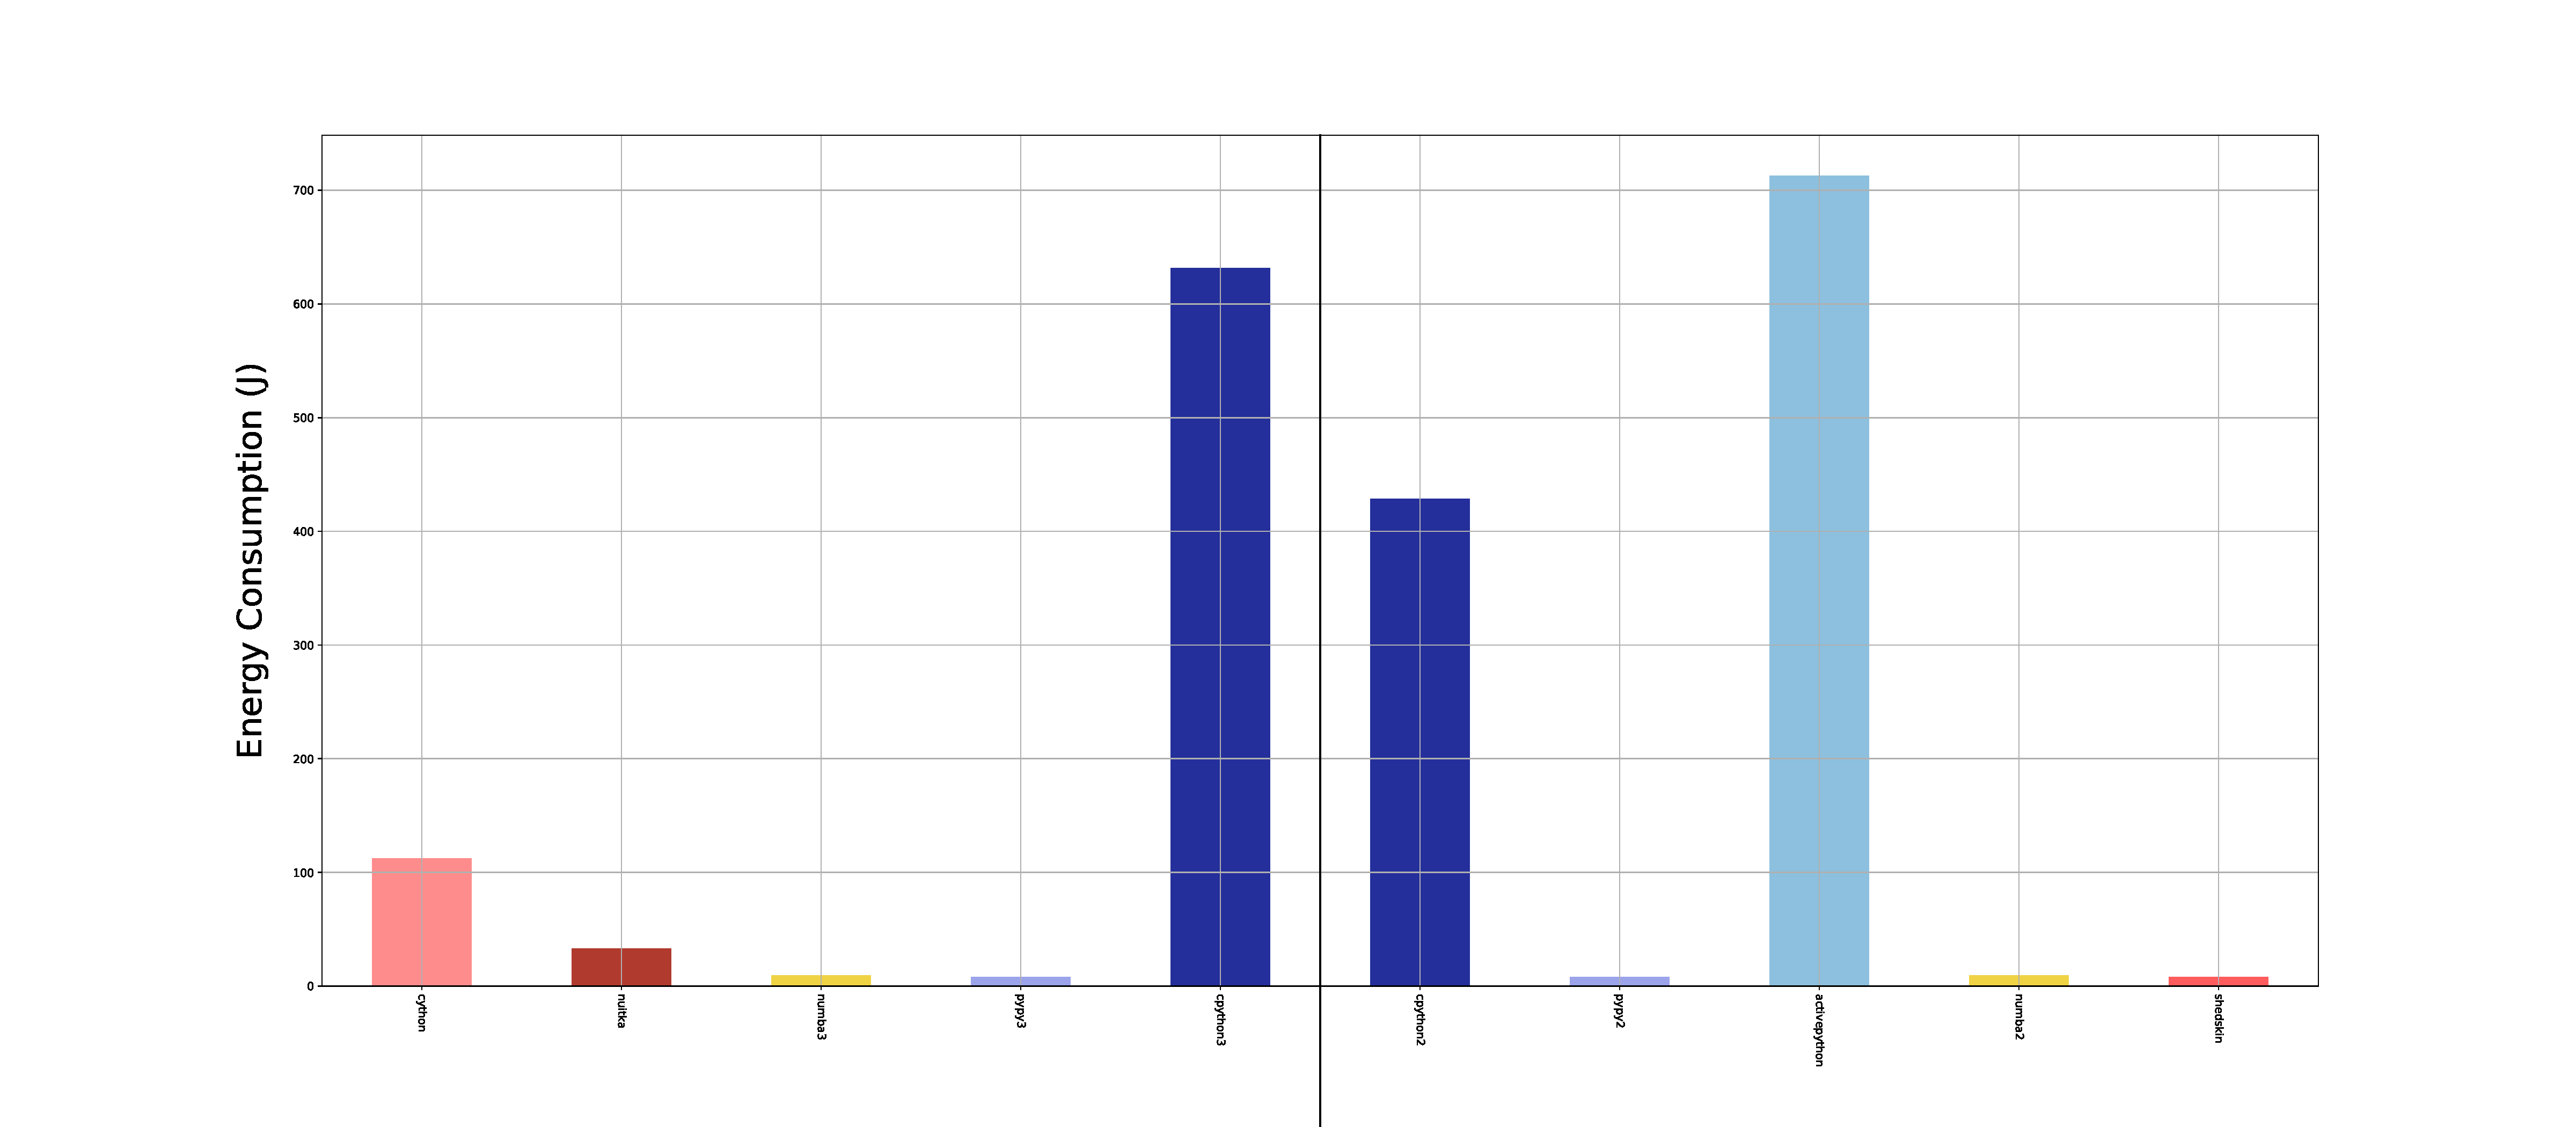
\includegraphics[width=\linewidth]{imgs/bitopts_mean}
      \caption{Summary of the binary operations for different python implementations }
      \label{fig:bitops}
\end{figure}

Figure~\ref{fig:bitops} depicts the average energy consumption of different implementations for the binary operations.
One can notice 3 clusters.
The first, which is the interpreted one, uses approximately 500 Joules per operation.
The second is a non-optimized compilation that includes Cython and Nuitka and uses 10 times less energy than the first.
And the final one, which has been fully optimized, uses 50 percent less energy. This category includes JIT libraries, also known as Numba, Python implementations that include JIT, also known as PyPy, and Shedskin, which transpile the source code into C and then use a C/C++ compiler to generate the binary, as opposed to Cython and Nuitka, which directly compile the Python code.
To conclude this experiment, JIT has a huge impact when it comes to binary operations, and an inadequate runtime selection can lead to a 100x increase in energy consumption.
Furthermore, we observed that different binary operations exhibit the same energy footprint for all the implementations, except Cython.

\section{Conclusion}
One can conclude that the choice of Python interpreter has a significant impact on the programs' energy consumption.
This investigation is made more intriguing by the absence of a universal solution.
The primary downside is the incompatibility of some of these solutions, which causes us to make concessions when we need a generic answer.
